\chapter{Extensions to the Neural Engineering Framework}
\label{chapt:nef-extensions}

Rapid growth in the field of neuromorphic engineering---over the past 30 years~\citep{mead1988silicon}---has accelerated the production of a large variety of neuromorphic architectures, each with distinct constraints and trade-offs that impact the degree of programmability and performance as a function of energy-consumption (section~\ref{sec:neuromorphic}).
Among these considerations, are issues involving:
discretization (in time), quantization (truncation of both neural states and weight matrices), connectivity constraints, memory constraints, volume of spike traffic, external input-output bandwidth and delays, thermal variability, transistor mismatch, conversion of analog signals to digital pulses, and the introduction of higher-order dynamics throughout.
The NEF already solves many of these problems in theory with varying degrees of success in practice.
The focus of this chapter is to expose our novel contributions to solving these problems in the context of extending the scope of Principle~3.
The intent is to bolster up the NEF with a variety of additional methods and techniques for analyzing and leveraging spiking dynamical computations.

\section{Synapses}
\label{sec:synaptic-extensions}

This section has been adapted from the works of \citet[][patent pending]{dynamicspatent}, \citet{voelker2017iscas}, \citet{voelker2017neuromorphic}, and \citet{voelker2018}.
Here, we focus on a dynamical primitive of SNNs known as the synapse model, $h(t)$, and address many of the differences that emerge between the idealization made by the NEF and the realities imposed by neuromorphic hardware (and often too, the brain).
This leads to several high-level results that exploit their higher-order dynamics, account for time-constant mismatch, leverage their heterogeneity, and solve for optimal filters.

\subsection{Linear transfer functions}
\label{sec:linear-extensions}

We build a comprehensive theory, adapted from \citet{voelker2018}, for including arbitrary linear synapse models in the neural architecture.
This is applied to the case of implementing linear systems, but many of these same techniques also carry over to later sections in the case of nonlinear systems. % the case of nonlinear dynamical systems with heterogeneous synapses~\citep{voelker2017iscas, voelker2017neuromorphic}.

Consider the linear time-inviant~(LTI) system (repeating equation~\ref{eq:lti}, for clarity):
\begin{equation} \label{eq:lti-repeated}
\begin{split}
\dot{\V{x}}(t) &= A\V{x}(t) + B\V{u}(t) \\
\V{y}(t) &= C\V{x}(t) + D\V{u}(t) \text{.}
\end{split}
\end{equation}
This state-space model is related to its \emph{transfer function}, $F(s)$, which uniquely characterizes its input-output response in the Laplace domain according to
$$
F(s) = \laplace{f(t)}(s) = \frac{\laplace{\V{y}(t)}(s)}{\laplace{\V{u}(t)}(s)} = \frac{\V{Y}(s)}{\V{U}(s)} \text{,}
$$
by the following equation~\citep{brogan1982modern}:
\begin{align} \label{eq:ss2tf}
F(s) = C(sI - A)^{-1}B + D \text{.}
\end{align}
Now let $F(s)$ be the transfer function for the linear dynamics that we wish to implement (derived by equations~\ref{eq:lti-repeated} and~\ref{eq:ss2tf}), and let $H(s)$ be the transfer function for an arbitrary linear synapse model ($H(s) = \mathcal{L} \left\{ h(t) \right\}$).
As stated in section~\ref{sec:principle3}, introducing the synapse model means replacing the integrator ($s^{-1}$) with $H(s)$.
This is equivalent to replacing $s$ with $H(s)^{-1}$.
Notably, substituting $H(s)$ for the integrator results in the transfer function $F \left( H(s)^{-1} \right)$, which no longer implements the original, desired dynamics $F(s)$. %, via the change-of-variables $s \longleftrightarrow H(s)^{-1}$.
However, we would like to ensure that the new dynamics match the originally specified $F(s)$.
The key insight is that we can determine a new function, $F^H(s)$, such that $F^{H}\left( H(s)^{-1} \right) = F(s)$.
That is, we can solve for a function that provides the original dynamics when implemented using the transfer function $H(s)$ as the dynamical primitive.
This is formalized by the following definition:
\begin{definition} \label{def:maps-onto}
A function $F^{H}(s)$ \emph{maps $F$ onto $H$} if and only if it satisfies:
\begin{align} \label{eq:maps-onto}
F^{H}\left( \frac{1}{H(s)} \right) = F(s) \text{.}
\end{align}
\end{definition}

This definition compactly expresses the notion of a ``change of dynamical primitive'', in that $F(s)$ is mapped from the canonical primitive, $s^{-1}$, onto some new primitive, $H(s)$.
Trivially, $F(s)$ maps itself onto $s^{-1}$.
Non-trivial examples are given below.
%To see this, we apply the key insight to some $F^{H}(s)$ to reveal that substituting the integrator for the synapse results in the dynamics $F^{H}(H(s)^{-1})$, which is equal to $F(s)$ if and only if it maps $F$ onto $H$, by definition~\ref{def:maps-onto}.
%Then, to compensate for this change in dynamics, we must solve for some transfer function $F^{H}(s)$ that satisfies definition~\ref{def:maps-onto}.
%This effectively means inverting the change-of-variables $s \longleftrightarrow H(s)^{-1}$.

Once we identify a $F^{H}(s)$ that maps $F$ onto $H$, any state-space model $\left( A^H\text{,}\, B^H\text{,}\, C^H\text{,}\, D^H \right)$ that satisfies
\begin{equation} \label{eq:ss-mapped}
F^{H} \left( s \right) = C^H \left( sI - A^H \right)^{-1}B^H + D^H
\end{equation}
will implement the desired dynamics when using $H(s)$ as the dynamical primitive, by equations~\ref{eq:ss2tf} and~\ref{eq:maps-onto} (see Figure~\ref{fig:lti-system-mapped-general}).

\begin{figure}
  \centering
  \resizebox{\columnwidth}{!} {
	\begin{tikzpicture}[auto, node distance=2cm,>=latex']
	  \node [input, name=input] {};
	  \node [coordinate, name=fanin, right of=input] {};
	  \node [block, right of=fanin, node distance=1.5cm] (B) {$B^H$};
	  \node [sum, right of=B, node distance=2cm] (sum) {$+$};
	  \node [block, right of=sum, node distance=2cm] (integ) {$H(s)$};
	  \node [block, right of=integ, node distance=3.5cm] (C) {$C^H$};
	  \node [sum, right of=C, node distance=2cm] (sumout) {$+$};
	  \node [output, right of=sumout] (output) {};
	
	  \node [block, below of=integ] (A) {$A^H$};
	  \node [block, above of=integ] (D) {$D^H$};
	
	  \draw [-] (input) -- node {$\V{u}$} (fanin);
	  \draw [->] (fanin) -- node {} (B);
	  \draw [->] (fanin) |- (D);
	  \draw [->] (D) -| node {} (sumout);
	  \draw [->] (B) -- node {} (sum);
	  \draw [->] (sum) -- node {} (integ);
	  \draw [->] (integ) -- node [name=fanout] {$\V{x}$} (C);
	  \draw [->] (fanout) |- (A);
	  \draw [->] (A) -| node {} (sum);
	  \draw [->] (C) -- node {} (sumout);
	  \draw [->] (sumout) -- node {$\V{y}$} (output);
	\end{tikzpicture}  
  }
  \caption[Extending Principle~3 to arbitrary linear synapses.]{ \label{fig:lti-system-mapped-general}
    Block diagram for an LTI system, equivalent to Figure~\ref{fig:lti-system}, with the integrator replaced by a more general linear filter $H(s)$.
    The state-space model $\left( A^H\text{,}\, B^H\text{,}\, C^H\text{,}\, D^H \right)$ is obtained from some transfer function $F^{H}(s)$ that maps $F$ onto $H$, as defined in the text.
    This generalizes Figure~\ref{fig:lti-system-mapped} to arbitrary linear synapse models.
    Reproduced from \citet[][Figure~7]{voelker2018}.
  }
\end{figure}

Therefore, supposing $F^{H}(s)$ satisfies definition~\ref{def:maps-onto}, and that it is convertible to a state-space model (equation~\ref{eq:lti}), then Figure~\ref{fig:lti-system-mapped-general} is just another form of Figure~\ref{fig:lti-system}, but with the integrator replaced by the synapse.
Note that this construction, on its own, does not specify how to find a satisfying $F^{H}(s)$, nor whether such a function exists, nor whether it can be converted to a state-space model.
We provide several examples leading to such a specification at the end of this section.
%This will be made clear through a number of examples, culminating with an approach that recovers an important result from linear systems theory (see appendix~\ref{app:discrete-connection}).
%In appendix~\ref{app:state-space} we discuss our freedom to choose state-space models, and the connection to choice of encoders in the NEF.

Before proceeding, we remark that the above theory directly carries over from the continuous-time domain to the discrete-time domain.
The discrete-time formulation of an LTI system is similar to equation~\ref{eq:lti}, but increments time in steps of length $\dt{}$:
\begin{equation} \label{eq:dlti}
\begin{split}
\V{x}[t+\dt{}] &= \bar{A}\V{x}[t] + \bar{B}\V{u}[t] \\
\V{y}[t] &= \bar{C}\V{x}[t] + \bar{D}\V{u}[t] \text{,}
\end{split}
\end{equation}
where the discrete state-space model $\left( \bar{A}\text{,}\, \bar{B}\text{,}\, \bar{C}\text{,}\, \bar{D} \right)$ fully defines the system.
The discrete-time equivalent to the Laplace transform is the $\mathcal{Z}$\emph{-transform}, named for its use of the variable $z$ to denote the complex frequency domain.
In this domain, $z^{-1}$ plays the role of $s^{-1}$, by performing a discrete shift forwards, one step in time (i.e.,~a delay of one time-step), instead of integration.
A well-known result is that the transfer function of this discrete LTI system---defined as the ratio of the $\mathcal{Z}$-transform of the output to the $\mathcal{Z}$-transform of the input---is equal to $F(z) = \bar{C} (zI - \bar{A})^{-1} \bar{B} + \bar{D}$, analogously to equation~\ref{eq:ss2tf}.
Consequently, all of the previous discussion carries over to discrete LTI systems.
In particular, for a discrete synapse expressed using the $\mathcal{Z}$-transform, $H(z)$, we have the analogous definition:
\begin{definition} \label{def:discrete-maps-onto}
A function $F^{H}(z)$ \emph{maps $F$ onto $H$} if and only if it satisfies:
\begin{align} \label{eq:discrete-maps-onto}
F^{H}\left( \frac{1}{H(z)} \right) = F(z) \text{.}
\end{align}
\end{definition}
Given some $F^{H}(z)$ that maps $F$ onto $H$, any state-space model $\left( \bar{A}^H\text{,}\, \bar{B}^H\text{,}\, \bar{C}^H\text{,}\, \bar{D}^H \right)$ that satisfies
\begin{equation} \label{eq:dss-mapped}
F^{H} \left( z \right) = \bar{C}^H \left( zI - \bar{A}^H \right)^{-1}\bar{B}^H + \bar{D}^H
\end{equation}
will implement the desired dynamics $F(z)$ when using $H(z)$ as the dynamical primitive.
Hence, the task of determining $F^{H}(\cdot)$ is identical for both continuous- and discrete-time domains---it is only $F(\cdot)$ and $H(\cdot)$ that differ.

\subsubsection{Continuous lowpass synapse}

The first example we consider demonstrates that our new theory recovers the standard form of Principle~3 from the NEF (see section~\ref{sec:principle3}).
For the case of a continuous-time first-order lowpass filter (equation~\ref{eq:lowpass}), $H(s) = \left(\tau s + 1 \right)^{-1}$, let:
\begin{align*}
F^H(s) &:= C \left( sI - (\tau A + I) \right)^{-1} \left( \tau B \right) + D \\
&= C \left( \left(\frac{s-1}{\tau}\right)I - A \right)^{-1}B + D \text{.}
\end{align*}
Then, 
\begin{align*}
F^H \left( \tau s + 1 \right) &= C \left( \left(\frac{(\tau s + 1) - 1}{\tau}\right) I - A \right)^{-1}B + D \\
&= F(s)\text{,} 
\end{align*}
which satisfies definition~\ref{def:maps-onto}.
Therefore, by equation~\ref{eq:ss-mapped},
\begin{equation} \label{eq:p3-novel}
\begin{aligned}
A^H &= \tau A + I \text{,} & \quad C^H &= C \text{,} \\
B^H &= \tau B \text{,} & \quad D^H &= D \text{.}
\end{aligned}
\end{equation}
%$A^H = \tau A + I$, $B^H = \tau B$, $C^H = C$, and $D^H = D$.
This completes our novel proof of Principle~3 from section~\ref{sec:principle3}.

\subsubsection{Discrete lowpass synapse}

When simulating any NEF network on a digital computer, we necessarily use time-steps of finite length $\dt{} > 0$ to advance the state of the network, updating at discrete moments in time~\citep{bekolay2014}.
For instance, Nengo currently uses a default of $\dt{} = 1$\,ms, and implements a zero-order hold~(ZOH) discretization of the synaptic filter.
Implementing ZOH means that all continuous-time signals are held constant within each time-step.
This discretization of equation~\ref{eq:lowpass} gives:
\begin{equation}
H(z) = \frac{1 - a}{z - a} \text{,} \quad a := e^{-\frac{\dt{}}{\tau}} \text{.} \nonumber
\end{equation}
If our desired transfer function is expressed in continuous-time, $F(s)$, then we should also discretize it to $F(z) = \bar{C} (zI - \bar{A})^{-1} \bar{B} + \bar{D}$, with the same time-step, and again using ZOH discretization for consistency.
Let,
\begin{align*}
F^H(z) &:= \bar{C} \left(zI - \frac{1}{1 - a} \left(\bar{A} - aI \right) \right)^{-1} \left( \frac{1}{1-a}\bar{B} \right) + \bar{D} \\
&= \bar{C} \left( \left(z(1 - a) + a \right)I - \bar{A} \right)^{-1}\bar{B} + \bar{D} \text{.}
\end{align*}
Then, 
\begin{align*}
F^H \left( \frac{z-a}{1-a} \right) &= \bar{C}\left( \left( \frac{z-a}{1-a}(1 - a) + a \right)I - \bar{A} \right)^{-1}\bar{B} + \bar{D} \\
&= F(z) \text{,}
\end{align*}
which satisfies definition~\ref{def:discrete-maps-onto}.
Therefore, by equation~\ref{eq:dss-mapped},\begin{equation} \label{eq:discrete-p3}
\begin{aligned}
\bar{A}^H &= \frac{1}{1 - a} \left(\bar{A} - aI\right) \text{,} & \quad \bar{C}^H &= \bar{C} \text{,} \\
\bar{B}^H &= \frac{1}{1-a}\bar{B} \text{,} & \quad \bar{D}^H &= \bar{D} \text{,}
\end{aligned}
\end{equation}
provides an exact implementation of the desired system for digital architectures, regardless of the simulation time-step (assuming ZOH).
% Consequently, we use this method in the simulations reported in this paper unless otherwise noted.

\subsubsection{Delayed continuous lowpass synapse}

Next, we consider a continuous-time first-order lowpass filter with a time-delay of $\lambda$:
\begin{equation} \label{eq:delayed-lowpass}
H(s) = \frac{e^{-\lambda s}}{\tau s + 1} \text{.}
\end{equation}
This same model has been proposed by \citet[][equation~6.2]{roth2009modeling} as a more realistic alternative to equation~\ref{eq:lowpass}, that includes an axonal transmission delay of length $\lambda$ (on the order of $\tau$) to account for the finite-velocity propagation of action potentials.
By commutativity of convolution, modeling the delay in the synapse (as in equation \ref{eq:delayed-lowpass}) is equivalent to modeling the delay in spike propagation.
Equation~\ref{eq:delayed-lowpass} may also be used to account for feedback delays within some broader setting (e.g.,~when the feedback term is computed via some delayed system).

In the mammallian cortex, $\lambda$ is known to range between $0.1$--$44$\,ms while being precise and reproducible~\citep{lagorce2015stick}.
In analog circuitry, $\lambda$ grows in proportion to the square of the wire length, and is necessarily introduced by the pulse-extension of digital-to-analog circuits~\citep{voelker2017iscas}.
This delay term may also be configured on digital architectures such as Loihi~\citep{davies2018loihi}.

Letting $d := \frac{\lambda}{\tau}e^{\frac{\lambda}{\tau}}$, and $W_0(\cdot)$ denote the principal branch of the Lambert-$W$ function~\citep{corless1996lambertw}, we invert $y := H(s)^{-1}$ as follows:
\begin{align*}
&& y &= \left(\tau s + 1\right) e^{\lambda s} && \\
\iff && \frac{\lambda}{\tau}e^{\frac{\lambda}{\tau}} y &= \left( \lambda s + \frac{\lambda}{\tau} \right) e^{\lambda s + \frac{\lambda}{\tau}} && \\
\iff && W_0(dy) &= \lambda s + \frac{\lambda}{\tau} && \\
\iff && \frac{1}{\lambda} W_0(dy) - \frac{1}{\tau} &= s \text{,} &&
\end{align*}
where the second-last line assumes that $|\eta| < \pi$ and $\lambda \text{Re}\left[ s \right] + \frac{\lambda}{\tau} > - \eta \cot \eta$, where $\eta := \lambda \text{Im}\left[ s \right]$, in order for $\lambda s + \frac{\lambda}{\tau}$ to be within the principal branch~\citep[][equation~4.4]{corless1996lambertw}.\footnote{%
A simpler (but only sufficient) condition is $\text{Re} \left[ s \right] \ge -\frac{1}{\tau}$ and $ | \text{Im} \left[ s \right] | < \frac{\pi}{2 \lambda}$.
Thus, it suffices to consider input frequencies $< \frac{1}{4\lambda}$\,Hz.}
Therefore,
\begin{align}
&& F^H(s) &:= F\left( \frac{1}{\lambda} W_0(ds) - \frac{1}{\tau} \right) \label{eq:delayed-lowpass-mapped} && \\
\implies && F^H(H(s)^{-1}) &= F^H(y) = F(s) \text{.} && \nonumber
\end{align}

As a demonstration of how we might use this mapping, suppose the desired transfer function for our system is a time-delay of $\theta$ seconds, $F(s) = e^{-\theta s}$ (equation~\ref{eq:tf-delay}).
In this setting, we are attempting to ``amplify'' a delay of $\lambda$ seconds in the synapse into a system delay of $\theta$ seconds at the network level.
Letting $c := e^{\frac{\theta}{\tau}}$ and $r := \frac{\theta}{\lambda}$, and then substituting $F(s)$ into equation~\ref{eq:delayed-lowpass-mapped}, provides the required function:
\begin{align}
F^H(s) = \exp \left\{ -\theta \left( \frac{1}{\lambda} W_0(ds) - \frac{1}{\tau} \right) \right\} = c \exp \left\{-r W_0(ds) \right\} = c \left( \frac{W_0(ds)}{ds} \right)^r \text{.} \nonumber
\end{align}
This may be numerically converted into a state-space model, of arbitrarily chosen dimensionality $q$, via the $\left[q-1/q\right]$ Pad\'e approximants of the following Maclaurin series:
\begin{align} \label{eq:lambert-delay}
F^H(s) = c r \sum_{i=0}^\infty \frac{(i+r)^{i-1}}{i!} (-ds)^i \text{.}
\end{align}
To our knowledge, there is no closed-form expression for the Pad\'e approximants of equation~\ref{eq:lambert-delay}, but there are methods to compute them accurately and in $\bigoh{q^2}$ time~\citep{sidi2003practical}.
Given these approximants, we may follow the same procedure that we use in section~\ref{sec:nef-delay} (see equation~\ref{eq:pade}) to obtain an LTI system in the form of equation~\ref{eq:lti}.
In section~\ref{sec:pure_delay}, we use this approach to improve the accuracy of the delay network demonstrated in section~\ref{sec:nef-delay}. %(see~Figure~\ref{fig:lambert}).
We remark that each of $d$, $c$, and $r$ are dimensionless (i.e.,~unitless) constants that can be used to relate measurable properties of a biological system that may be governed by this description to the necessary network-level computations.

\subsubsection{Coordinate transformation}

Before proceeding with the general solution, we introduce some useful intermediate results:
\begin{lemma}[Transforming coordinates between dynamical systems] \label{lemma:coord-transform}
Let $\V{f}(t)$ and $\V{g}(t)$ be infinitely time-differentiable signals, that are related by:
\begin{equation} \label{eq:f}
\V{f} = \sum_{i=0}^\infty c_i \V{g}^{(i)} \text{,}
\end{equation}
for some coordinates $\coords{c}{i}$. Then this dynamical system is equivalent to:
\begin{equation} \label{eq:g}
\V{g} = \sum_{i=0}^\infty b_i \V{f}^{(i)} \text{,}
\end{equation}
where the coordinates $\coords{b}{i}$ are defined by the recursive transformation:
\begin{equation} \label{eq:b}
b_i = c_0^{-1} \begin{cases}
    1 & i = 0 \\
    %- (b \ast c)\left[ i \right] & i \ge 1 ,
    - \sum_{j=0}^{i-1} b_j c_{i - j} & i \ge 1 \text{.}
  \end{cases}
\end{equation}
%and $(b \ast c)\left[ i \right] := \sum_{j=0}^{i-1} b_j c_{i - j}$ is a discrete convolution. % that depends on $b_j$ for all $0 \le j \le i - 1$.
\end{lemma}

\begin{corollary}
\label{cor:coord-transform}
Let: $$H_c(s) = \frac{1}{\sum_{i=0}^\infty c_i s^i}, \quad H_b(s) = \frac{1}{\sum_{i=0}^\infty b_i s^i}, $$ where $b$ is defined by equation~\ref{eq:b}. Then equation~\ref{eq:f} is equivalent to $F(s)H_c(s) = G(s)$ and similarly equation~\ref{eq:g} is equivalent to $G(s)H_b(s) = F(s)$, and moreover:
\begin{equation} \label{eq:inv}
H_c(s) H_b(s) = 1 \text{,}
\end{equation}
hence $H_c(s)$ and $H_b(s)$ are eachother's reciprocals. Furthermore, the coordinate transformation equation~\ref{eq:b} is its own inverse.
\end{corollary}

\begin{proof}
Noting that $\V{g}^{(0)} = \V{g}$, rearrange equation~\ref{eq:f} as:
\begin{equation} \label{eq:gf}
\V{g} = c_0^{-1} \V{f} + \sum_{i=1}^\infty (-c_0^{-1} c_i) \V{g}^{(i)} \text{.}
\end{equation}
Differentiate each side an infinite number of times, to obtain the following set of equations that hold for all $j \in \mathbb{N}$:
\begin{equation} \label{eq:dg}
\V{g}^{(j)} = c_0^{-1} \V{f}^{(j)} + \sum_{i=1}^\infty (-c_0^{-1} c_i) \V{g}^{(i+j)} \text{.}
\end{equation}
Now recursively substitute equation~\ref{eq:dg} into equation~\ref{eq:gf} for all occurrences of $\V{g}^{(i)}$, $i \ge 1$ until we are only left with $\V{f}^{(j)}$ terms for $j \le i$, and take the limit as $i \rightarrow \infty$. This is equivalent to treating equation~\ref{eq:dg} as a recursive function in $j$ and then evaluating $\V{g}^{(0)}$.
Although this is infinitely generative from a bottom-up perspective, we are `allowed' to do this because each substitution of equation~\ref{eq:dg} increases the order of $\V{g}$ by 1 (hence it terminates top-down). Another way to view this is we pick some finite $k$ in order to gather all occurrences of $\V{f}^{(k)}$ in the infinite expansion. After repeating this for all $k \rightarrow \infty$, we get something of the form:
\begin{equation*}
\V{g} = \sum_{k=0}^\infty \tilde{b}_k \V{f}^{(k)} \text{.}
\end{equation*}
Now, all that remains is to show that $\tilde{b}_k = b_k$ from equation~\ref{eq:b} in order to match equation~\ref{eq:g}. We do this inductively in a way that parallels the recursive structure of the substitution procedure.

For the base case ($k = 0$) it should be clear that $\tilde{b}_0 = c_0^{-1} = b_0$ since this is the only way to construct $\V{f}^{(0)}$.
For the inductive case ($k \ge 1$), the only way to construct $\V{f}^{(k)}$ is through the substitution of $\V{g}^{(k)}$ in equation~\ref{eq:dg}.
Furthermore, this occurs for all $0 \le j \le k - 1$. In particular, for every such $j$, we have the coefficient $(-c_0^{-1} c_{i})$ multiplied by $\V{g}^{(i + j)}$ to yield $c_0^{-1} \V{f}^{(k)}$ where $k = i + j$.
Finally, this occurs $\tilde{b}_{j} c_0$ times since it is mirrored by each occurrence of $\V{f}^{(j)}$.
Putting this all together, we get $\tilde{b}_k = \sum_{j=0}^{k-1} -c_0^{-1} c_{k - j} \tilde{b}_j = c_0^{-1} \sum_{j=0}^{k-1} - b_j c_{k - j} = b_k$ (by the inductive hypothesis).
\end{proof}

The coordinate transformation equation~\ref{eq:b} is equivalent to taking the Pad\'e approximants~\citep{Pade1892} for the special case of when the numerator is $p = 0$.
To be precise,
$$
\sum_{i=0}^{q} c_i x^i \approx \frac{1}{\sum_{i=0}^q b_i x^i}
$$
has the same optimal approximation from equation~\ref{eq:b} as taking the $[0/q]$~Pad\'e approximants:
$$
\coords{b}{i=0 \ldots q} = \left[ 0 / q \right] \sum_{i=0}^{q} c_i x^i \text{.}
$$
This can be seen through equation~\ref{eq:inv} and verified by comparing the algorithm for the extended Euclidean algorithm for the polynomial GCD, in this special case, to the algorithm equation~\ref{eq:b}. That is, they both implement long division.
We remark that the coordinate transformation equation~\ref{eq:b}---that is, the algorithm for finding the Pad\'e approximants when $p = 0$---is its own inverse. That is, we may convert back and forth using the same transformation without any loss of information.

We may also interpret equation~\ref{eq:b} as a discrete dynamical system by realizing that $b$ is the discrete convolution of itself with $c$. With some work, we can show that this is the same as stating that $\ztrans{b}\ztrans{c} = 1$, or equivalently in the time-domain, $\coords{b}{i=0\ldots q}$ is the impulse-response of the following discrete transfer function:
$$
H^q_{c \rightarrow b}(z) = \frac{z^{q}}{\sum_{i=0}^q c_i z^{q - i}} \text{,}
$$
and likewise, $H^q_{b \rightarrow c}(z)$ has the impulse-response $\coords{c}{i=0\ldots q}$.
Furthermore, $$\lim_{q \rightarrow \infty} H^q_{c \rightarrow b}(z) H^q_{b \rightarrow c}(z) = 1,$$ analogously to equation~\ref{eq:inv}.
Lastly, we note that the above Lemma and Corollary also apply to the case where differentials are replaced by discrete time-shifts and the Laplace transform is replaced by the $\mathcal{Z}$-transform.

\subsubsection{General linear synapse}

Finally, we consider the general class of all linear synapse models of the form:
\begin{equation} \label{eq:synapse}
H(s) = \frac{1 + \sum_{i=1}^p b_i s^i}{\sum_{i=0}^q \tilde{c}_i s^i} \text{,}
\end{equation}
%for some polynomial coefficients $\left( c_i \right)$ of arbitrary degree $k$.
That is, a rational function with real polynomial coefficients of potentially infinite order.
The only constraint is that $b_0 \ne 0$ (coefficients may be normalized to put it into this form where $b_0 = 1$).
This encompasses the class of nearly all linear filters, and, as far as we know, all linear synapse models used in the literature.
For instance, this includes the first-order lowpass synapse that is standard in the NEF.
It also includes the second-order alpha synapse, $(\tau s + 1)^{-2}$~\citep{rall1967distinguishing}---the convolution of two exponentials with identical time-constants---which is commonly used in biological models~\citep{koch1989methods, destexhe1994synthesis, mainen1995reliability, destexhe1998kinetic, roth2009modeling}.
The alpha synapse essentially filters the spike-trains twice, to produce PSCs with finite (non-instantaneous) rise-times.
In addition, equation~\ref{eq:synapse} includes a generalization of the alpha synapse, the double-exponential synapse, $(\tau_1 s + 1)^{-1}(\tau_2 s + 1)^{-1}$~\citep{wilson1989simulation}---the convolution of two exponentials with time-constants $\tau_1$ and $\tau_2$---which has different rise- and fall-times to account for the separate time scales of rapid transmitter binding followed by slow unbinding~\citep{destexhe1994synthesis, hausser1997estimating, roth2009modeling}.
The double-exponential is also a suitable model to account for parasitic capacitances in neuromorphic hardware~\citep{voelker2017iscas}.
Furthermore, equation~\ref{eq:synapse} includes a higher-order generalization of the alpha synapse, the gamma kernel, $(\mu^{-1} s + 1)^{-k}$~\citep[][equation 19]{de1992gamma}. 
Finally, this class contains more exotic models, such as the $Q$-bandpass synapse model, $({\omega^2}s^2 + (\omega Q)^{-1}s + 1)^{-1}$, where $\omega$ is the peak frequency in radians per second, and $Q$ is inversely proportional to the bandwidth.
Such synapses have been used to model bandpass filtering from mechanoreceptors in the fingertip~\citep{voelker2016a} or from rods in the retina~\citep{armstrong2003bandpass}.

As well, in the following section we demonstrate that equation~\ref{eq:synapse} may be used to model synapses with pure delays, which proves a complete connection to ZOH discretization.
%Within the NEF, both the alpha and double-exponential have the advantage of filtering the neural activity twice, thus reducing the spike-noise relative to the first-order lowpass.  CE: just didn't fit well anymore.
%Specifically, by the use of Pad\'e approximants, we may rewrite any transfer function with a Taylor series expansion (even those that are irrational or improper) in the form of equation~\ref{eq:synapse-rewritten}---albeit with some radius of convergence.
This same technique permits us to model, for instance, synapses with pulse-extended responses~\citep{voelker2017iscas}.
%\footnote{%
%Pad\'e approximants are computed ``manually'' by \citet[][equations~9--11]{voelker2017iscas} to obtain a second-order approximation in the form of equation~\ref{eq:synapse}.
Similarly, the delayed lowpass (equation~\ref{eq:delayed-lowpass}) may be expressed in the form of equation~\ref{eq:synapse}.
% Therefore, equation~\ref{eq:synapse} captures a wide variety of linear postsynaptic responses to some desired degree of accuracy.
Finally, any linear combinations of the aforementioned synapse models will also be a member of this class.
Nonlinear synapse models, such as conductance-based synapses~\citep[e.g.,][equation~6]{destexhe1994efficient}, are the active subject of study in the NEF~\citep{stockel2017, stoeckel2018}.

%It is interesting to note that although our characterization does not include nonlinear synapse models, such as conductance-based synapses~\citep[][equation~6]{destexhe1994efficient}, recent results indicate that, at least in some common cases, such models may also be accounted for without significantly impacting overall accuracy~\citep{stockel2017}.
%However, these results remain to be thoroughly tested and quantified.

The first step is to apply Corollary~\ref{cor:coord-transform} to the numerator $\{b\}_{i=0}^p$ in order to rewrite the transfer function in the following form:
\begin{equation} \label{eq:synapse-rewritten}
H(s) = \frac{1}{\sum_{i=0}^k c_i s^i} \text{,}
\end{equation}
where $k$ is potentially infinite. Now we state and prove the main theorem of this section.

\begin{theorem}[General state-space solution to leverage postsynaptic currents]
\label{thm:general-linear}
To map $F$ onto equation~\ref{eq:synapse-rewritten}, we let: %we begin by defining our solution to $F^{H}(s)$ in the form of its state-space model (see equation~\ref{eq:ss-mapped}):
\begin{equation} \label{eq:general-linear}
\begin{aligned}
A^H &= \sum_{i=0}^k c_i A^i \text{,} & \quad C^H &= C \text{,} \\
B^H &= \left( \sum_{j=0}^{k-1} s^j \sum_{i=j+1}^k c_i A^{i-j-1} \right) B \text{,} & \quad D^H &= D \text{.}
\end{aligned}
\end{equation}
This satisfies the required identity, $F^{H}(H(s)^{-1}) = F(s)$ (equation~\ref{eq:maps-onto}).
\end{theorem}

\begin{proof}
\begin{align*}
\left( \sum_{j=0}^{k-1} s^j \sum_{i=j+1}^k c_i A^{i-j-1} \right) (sI - A)  &= \sum_{j=0}^{k-1} \sum_{i=j+1}^k s^j c_i A^{i-j-1} (sI - A) \\
&= \sum_{i=0}^{k} \sum_{j=0}^{i-1} s^j c_i A^{i-j-1} (sI - A)  \\
%&= \sum_{i=0}^k c_i (sI - A) \sum_{j=0}^{i-1} s^j A^{i-j-1} \\
&= \sum_{i=0}^k c_i \left( \sum_{j=0}^{i-1} s^{j+1} A^{i - (j + 1)} - s^j A^{i - j} \right) \\
&= \sum_{i=0}^k c_i \left( s^i A^{i - i} - s^0 A^{i-0} \right) \\
&= \left( \sum_{i=0}^k c_i s^i \right) I - \sum_{i=0}^k c_i A^i \\
&= H(s)^{-1}I - A^H \text{.}
\end{align*}
We then complete the proof by substituting this result and the state-space model into our expression for the mapped transfer function from equation~\ref{eq:ss-mapped}:
\begin{align*}
F^H(H(s)^{-1}) &= C^H(H(s)^{-1}I - A^H)^{-1} B^H + D^H \\
&= C(H(s)^{-1}I - A^H)^{-1} \left( \sum_{j=0}^{k-1} s^j \sum_{i=j+1}^k c_i A^{i-j-1} \right) B + D \\
&= C(sI - A)^{-1} B + D \\
&= F(s) \text{.}
\end{align*}
\end{proof}

An alternative derivation may also be found in section~\ref{sec:nonlinear-extensions}. % \citet[][section~2.2]{voelker2017neuromorphic}.
An interesting insight gained with this solution is that it is not, in general, the case that $B^H$ is time-invariant, since it depends on the time-differential, $s$, for values of $k \ge 2$.
As a result, solutions will often not be a typical state-space model in the form of equation~\ref{eq:lti}.

Nevertheless, such solutions can still be implemented, as is, in practice.
Since $s^j$ is the $j^{\text{th}}$-order differential operator, this form of $B^H$ states that we must supply the $j^{\text{th}}$-order input derivatives $\V{u}^{(j)}$, for all $j = 1 \ldots k - 1$.
When $k = 1$, this is trivial (no derivatives are needed).
For $k \ge 2$, let us first define $B^H_j:= \left( \sum_{i=j+1}^k c_i A^{i-j-1} \right) B$.
Then equation~\ref{eq:general-linear} shows that the ideal state-space model must implement the input transformation as a linear combination of input derivatives, $\sum_{j=0}^{k-1} B^H_j \V{u}^{(j)}$.
If the derivatives of the input are available to the model, then the $F^{H}(s)$ we described may be used to precisely implement the desired $F(s)$.

However, if the required derivatives are not included in the neural representation, then it is natural to use a ZOH method by assuming $\V{u}^{(j)} = 0$, for all $j = 1 \ldots k - 1$:
\begin{equation} \label{eq:general-linear-approx}
B^H = B^H_0 =  \left( \sum_{i=1}^k c_i A^{i-1} \right) B \text{,}
\end{equation}
with $A^H$, $C^H$, and $D^H$ as before (see equation~\ref{eq:general-linear}).
This is now an equivalent model to equation~\ref{eq:general-linear} assuming ZOH, and in the form of the standard state-space model (equation~\ref{eq:lti}).
In section~\ref{sec:derivatives}, we characterize the dynamics of this new system in terms of $F$ and $H$ (independently of the chosen state-space model) for general inputs.
We find that equation~\ref{eq:general-linear-approx} adds $k - 1$ new dimensions, for every dimension in $F$, to the state underlying the resulting dynamical system.
In the following section, we show that the our results yield a novel derivation of ZOH discretization for LTI systems.

To our knowledge, this specific state-space architecture has not been explored in theory or in practice.
Given that equation~\ref{eq:general-linear} requires the input derivatives to accurately compute low-dimensional network-level dynamics, this strongly suggests that it is important to represent and compute derivatives in neural systems.
Methods of computing derivatives have been explored by \citet{tripp2010} within the NEF.
As well, it has long been suggested that adaptive neural mechanisms (e.g., synaptic depression or spike-rate adaptation) may also play a fundamental role in computing such derivatives~\citep{abbott2004synaptic, lundstrom2008fractional}.
However, there has typically been less emphasis placed on understanding temporal differentiation in comparison to other temporal operators, such as integration~\citep{tripp2010}.

Finally, we again note that these results translate directly to the discrete-time domain.
The required state-space matrices are the same as in equation~\ref{eq:general-linear}, but with $\left( \bar{c}_i \right)$ corresponding to the coefficients of $H(z)$, bars affixed to each state-space matrix, and $z$ substituted for $s$ in $\bar{B}^H$.
However, the $z^j$ operator is a shift backwards by $j$ time-steps (i.e.,~an acausal lookahead), and so the ZOH assumption is instead $\V{u}[t+j\dt{}] = \V{u}[t]$ for all $j = 1 \ldots k - 1$.
Thus, the discrete analog to equation~\ref{eq:general-linear-approx} is:
\begin{equation} \label{eq:general-linear-approx-discrete}
\bar{B}^H = \left( \sum_{j=0}^{k-1} \sum_{i=j+1}^k \bar{c}_i \bar{A}^{i-j-1} \right) \bar{B} \text{.}
\end{equation}

\subsubsection{Relationship to discretization}

There is an interesting connection between definition~\ref{def:maps-onto} and the well-known problem of discretizing a linear dynamical system.
A discrete LTI system (equation~\ref{eq:dlti}) is identical to a continuous LTI system (equation~\ref{eq:lti}), with three adjustments: (1)~the integrator $s^{-1}$ is replaced by a time-delay of $\dt{}$ seconds, (2)~the input signal is sampled every $\dt{}$ seconds, and (3)~the output signal is sampled every $\dt{}$ seconds.
Focusing on point~1, this is precisely the notion captured by definition~\ref{def:maps-onto} with respect to:
\begin{equation*}
H(s) = e^{-\dt{}s} = \frac{1}{e^{\dt{}s}} = \frac{1}{\sum_{i=0}^\infty \frac{\dt{}^i}{i!} s^i} \text{,}
\end{equation*}
by the Maclaurin series of $e^{x}$.
That is, a synapse model that represents a pure delay of $\lambda = \dt{}$ without any additional filtering.
This is in the form of equation~\ref{eq:synapse-rewritten} with $c_i = \frac{\dt{}^i}{i!}$ as $k \rightarrow \infty$.
These coefficients are also the $\left[ 0 / \infty \right]$ Pad\'e approximants of $\sum_{i=0}^\infty \frac{(-\dt{})^i}{i!} s^i$, and likewise the result of the coordinate transformation equation~\ref{eq:b}.

If we make the ZOH assumption---that the input signal is held piecewise-constant over each continuous-time interval of length $\dt{}$---then $\V{u}^{(j)} = 0$ for all $j \ge 1$.
Therefore, by equation~\ref{eq:general-linear-approx}, an equivalent state-space model is:
\begin{align*}
A^H &= \sum_{i=0}^k c_i A^i = \sum_{i=0}^k \frac{\left(A\dt{}\right)^i}{i!} = e^{A\dt{}} \text{,} & C^H &= C \text{,} \\
B^H &= \left( \sum_{i=1}^k c_i A^{i-1} \right) B = A^{-1} \left(A^H - I\right) B \text{,} & D^H &= D \text{,}
\end{align*}
which is precisely the discrete state-space model $(\bar{A}, \bar{B}, \bar{C}, \bar{D})$ obtained by ZOH discretization~\citep{brogan1982modern}.
The discrete signals in equation~\ref{eq:dlti} correspond with points~2 and~3.

This connection helps to illustrate the scope and consistency of our theory.
In particular, the important procedure of discretizing linear state-space models may be viewed as a special case of accounting for changes in dynamical primitives.
Furthermore, as one should hope, the ZOH assumption recovers the correct result, which is normally proven by integrating the linear differential equations over the interval $[0\text{,}\, \dt{}]$.

\subsection{Nonlinear state-spaces}
\label{sec:nonlinear-extensions}

This section has been adapted from the work of \citet{voelker2017iscas}, which in turn extends the work of \citet{voelker2017neuromorphic} in applying the NEF to the mixed-signal synapses of Braindrop~\citep{braindrop2019}.
Here we derive two theorems for nonlinear systems, by taking a subtly different perspective than that of the previous section.
This generalizes the approach taken in \citet{voelker2017neuromorphic}, which considered the special case of a pulse-extended (i.e.,~time-delayed) double-exponential synapse.
%, which was inspired by Wilten Nicola's phase-space derivation of Principle~3 with double exponential synapses for autonomous systems [personal communication].

We wish to implement some desired nonlinear dynamical system,
\begin{equation} \label{eq:nonlinear}
\dot{\V{x}}(t) = f(\V{x}, \V{u}) \text{,}
\end{equation}
using equation~\ref{eq:synapse-rewritten} (rewritten from the form of equation~\ref{eq:synapse}) as the synaptic filter, $h(t)$.
Letting $\V{w}(t) = f^h(\V{x}, \V{u})$ for some recurrent function $f^h$ and observing that $\V{x}(t) = (\V{w} \ast h)(t)$, we may express these dynamics in the Laplace domain:
\begin{align*}
&& \frac{\V{X}(s)}{\V{W}(s)} &= \frac{1}{\sum_{i=0}^k c_i s^i} \\
\iff && \V{W}(s) &= \V{X}(s) \sum_{i=0}^k c_i s^i = \sum_{i=0}^k c_i \left[ s^i \V{X}(s) \right] \\
\iff && \V{w}(t) &= \sum_{i=0}^k c_i \V{x}^{(i)}
\end{align*}
since $s$ is the differential operator. This proves the following theorem:
\begin{theorem}[Nonlinear solution to leverage continuous postsynaptic currents] \label{thm:p3cont-nonlinear}
Let the function computed along the recurrent connection be:
\begin{align}
f^h(\V{x}, \V{u}) = \sum_{i=0}^k c_i \V{x}^{(i)}
\end{align}
where $\V{x}^{(i)}$ denotes the $i^\text{th}$ time-derivative of $\V{x}(t)$, and $c_i$ are given by equation~\ref{eq:synapse-rewritten}. Then the resulting dynamical system is precisely equation~\ref{eq:nonlinear}.
\end{theorem}

For the discrete case, we begin with some desired nonlinear dynamics expressed over discrete time-steps:
\begin{equation} \label{eq:disc-nonlinear}
\V{x}[t+dt] = \bar{f}(\V{x}, \V{u}) \text{,}
\end{equation}
using equation~\ref{eq:synapse-rewritten} (with $s$ replaced by $z$; the coordinate transformation still applies) as the synaptic filter $h[t]$, followed by an analogous theorem:
\begin{theorem}[Nonlinear solution to leverage discrete postsynaptic currents] \label{thm:p3disc-nonlinear}
Let the function computed along the recurrent connection be:
\begin{align}
\bar{f}^h(\V{x}, \V{u}) = \sum_{i=0}^k \bar{c}_i \V{x}^{[i]}
\end{align}
where $\V{x}^{[i]}$ denotes the $i^\text{th}$ discrete forwards time-shift of $\V{x}$, and $\bar{c}_i$ are likewise read from the denominator of $H(z)$.
Then the resulting dynamical system is precisely equation~\ref{eq:disc-nonlinear}.
\end{theorem}
The proof for the discrete case is nearly identical.
For sake of completeness, let $\V{w}[t] = \bar{f}^h(\V{x}, \V{u})$ for some recurrent function $\bar{f}^h$ and observe that $\V{x}[t] = (\V{w} \ast h)[t]$:
\begin{align*}
&& \frac{\V{X}(z)}{\V{W}(z)} &= \frac{1}{\sum_{i=0}^k \bar{c}_i z^i} \\
\iff && \V{W}(z) &= \V{X}(z) \sum_{i=0}^k \bar{c}_i z^i = \sum_{i=0}^k \bar{c}_i \left[ z^i \V{X}(z) \right] \\
\iff && \V{w}[t] &= \sum_{i=0}^k \bar{c}_i \V{x}^{[i]}
\end{align*}
since $z$ is the forwards time-shift operator. \qed

\subsubsection{Continuous lowpass synapse}

For standard Principle~3, we have $H(s) = \frac{1}{\tau s + 1}$ $\implies$ $k = 1$, $c_0 = 1$ and $c_1 = \tau$, 
\begin{equation} \label{eq:p3cont-nonlinear}
\implies f^h(\V{x}, \V{u}) = c_0 \V{x}^{(0)} + c_1 \V{x}^{(1)} = \V{x} + \tau \dot{\V{x}} = \tau f(\V{x}, \V{u}) + \V{x} \text{.}
\end{equation}
Note that equation~\ref{eq:p3cont-nonlinear} is consistent with equation~\ref{eq:p3-novel} and with Principle~3 from the NEF.

\subsubsection{Discrete lowpass synapse}

For the discrete case of Principle~3, we have $H(z) = \frac{1 - a}{z - a}$, where $a = e^{-\dt{} / \tau}$ $\implies$ $k = 1$, $\bar{c}_0 = -a(1 - a)^{-1}$, $\bar{c}_1 = (1 - a)^{-1}$,
\begin{equation} \label{eq:p3discrete-nonlinear}
\implies \bar{f}^h(\V{x}, \V{u}) = \bar{c}_0 \V{x}^{[0]} + \bar{c}_1 \V{x}^{[1]} =  (1 - a)^{-1}(\bar{f}(\V{x}, \V{u}) - a\V{x}) \text{.}
\end{equation}
Note that equation~\ref{eq:p3discrete-nonlinear} is consistent with equation~\ref{eq:discrete-p3}.

\subsubsection{Continuous double-exponential synapse}

For the double exponential synapse:
\begin{equation} \label{eq:double-exp}
H(s) = \frac{1}{(\tau_1 s + 1)(\tau_2 s + 1)} = \frac{1}{\tau_1 \tau_2 s^2 + (\tau_1 + \tau_2)s + 1}
\end{equation}
\begin{align} \label{eq:double-exp-solution}
\implies f^h(\V{x}, \V{u}) &= \V{x} + (\tau_1 + \tau_2) \dot{\V{x}} + \tau_1 \tau_2 \ddot{\V{x}} \nonumber \\
&= \V{x} + (\tau_1 + \tau_2) f(\V{x}, \V{u}) + \tau_1 \tau_2 \left( \frac{\partial f(\V{x}, \V{u})}{\partial \V{x}} \cdot f(\V{x}, \V{u}) + \frac{\partial f(\V{x}, \V{u})}{\partial \V{u}} \cdot \dot{\V{u}} \right) \text{.}
\end{align}
In the linear case, this simplifies to:
\begin{align*}
f^h(\V{x}, \V{u}) = \left( \tau_1 \tau_2 A^2 + (\tau_1 + \tau_2) A + I \right) \V{x} + \left( \tau_1 + \tau_2 + \tau_1 \tau_2 A \right) B \V{u} + \tau_1 \tau_2 B \dot{\V{u}} \text{.}
\end{align*}

\subsubsection{General linear synapses}

Consistent with what was found in section~\ref{sec:linear-extensions}, Theorems~\ref{thm:p3cont-nonlinear} and~\ref{thm:p3disc-nonlinear} require that we differentiate the desired dynamical system.
For the case of nonlinear systems, this means (if $k \ge 2$) determining the (possibly higher-order) Jacobians of $f$, as shown in equation~\ref{eq:double-exp-solution}.
For the special case of LTI systems, we can determine this analytically to obtain a closed-form expression.
By induction it can be shown that:
$$\V{x}^{(i)} = A^i\V{x} + \sum_{j=0}^{i-1} A^{i-j-1} B \V{u}^{(j)} \text{.}$$
Then by expanding and rewriting the summations:
\begin{align}
f^h(\V{x}, \V{u}) &= \sum_{i=0}^k c_i \V{x}^{(i)} \nonumber \\
&= \sum_{i=0}^k c_i \left[ A^i \V{x} + \sum_{j=0}^{i-1} A^{i-j-1} B \V{u}^{(j)} \right] \nonumber \\
&= \underbrace{\left( \sum_{i=0}^k c_i A^i \right)}_{\text{Recurrent
Matrix}}\V{x} + \sum_{j=0}^{k-1} \underbrace{\left( \sum_{i=j+1}^k c_i A^{i-j-1} \right)B}_{\text{Input Matrices}} \V{u}^{(j)} \text{.} \label{eq:p3general-lti}
\end{align}
The discrete case is identical:
\begin{align}
\bar{f}^h(\V{x}, \V{u}) = \underbrace{\left( \sum_{i=0}^k \bar{c}_i \bar{A}^i \right)}_{\text{Recurrent
Matrix}}\V{x} + \sum_{j=0}^{k-1} \underbrace{\left( \sum_{i=j+1}^k \bar{c}_i \bar{A}^{i-j-1} \right)\bar{B}}_{\text{Input Matrices}} \V{u}^{[j]} \text{.} \label{eq:p3general-lti-discrete}
\end{align}
This gives a matrix form for any LTI system with a $k^\text{th}$ order synapse, provided we can determine $\V{u}^{(j)}$ or $\V{u}^{[j]}$ for $0 \le j \le k-1$.
% Note that since $u$ and $x$ do not interact nonlinearly, we can separate them into input and recurrent transformations respectively, and only represent $x$ in the ensemble.
%For example, we can apply equation~\ref{eq:p3general-lti} to the double exponential synapse equation~\ref{eq:double-exp}:
%\begin{align*}
%f^h(\V{x}, \V{u}) = \, & (\tau_1 \tau_2 A^2 + (\tau_1 + \tau_2) A + I)\V{x} +  (\tau_1 + \tau_2 + \tau_1 \tau_2 A) B \V{u} + \tau_1 \tau_2 B \dot{\V{u}} \text{.}
%\end{align*}
Again, equation~\ref{eq:p3general-lti} is consistent with equation~\ref{eq:general-linear} and equation~\ref{eq:general-linear-approx}, as is equation~\ref{eq:p3general-lti-discrete} with equation~\ref{eq:general-linear-approx-discrete}.

\subsubsection{Pulse-extended double-exponential}

Finally, we show how this all connects to the higher-order dynamics of the pulse-extended double-exponential synapses in Braindrop~\citep{voelker2017iscas}.
Specifically, due to parasitic capacitances in the analog circuitry, a double-exponential ($\tau_1$, $\tau_2$) emerges, and, due to the pulse-extension from digital-to-analog (i.e.,~spike-to-synapse) conversion, a pulse is generated that is modelled as a box-filter with finite width, $\epsilon$, and height, $\gamma$.
This model is summarized by~\citet[][equation~8]{voelker2017iscas}:
\begin{equation} \label{eq:braindrop-synapse}
H(s) = \frac{ \gamma \left(1 - e^{-\epsilon s} \right) s^{-1}}{ \left( \tau_1 s + 1 \right) \left( \tau_2 s + 1 \right) }
\end{equation}
Now we apply lemma~\ref{lemma:coord-transform} in the following context:
$$
\V{f} = (\epsilon \gamma)^{-1} \left( \V{x} + (\tau_1 + \tau_2) \dot{\V{x}} + \tau_1 \tau_2 \ddot{\V{x}} \right) \text{,}
$$
$$
c_i = \frac{(-\epsilon)^i}{(i + 1)!} \text{,}
$$
where $\V{g}$ from the lemma is the signal that will be be used to drive the pulse-extender to satisfy $\V{f} = \sum_{i=0}^\infty c_i \V{g}^{(i)}$.
We now apply a fourth-order truncation to the coefficients:
$$
c_0 = 1, \quad c_1 = -\frac{\epsilon}{2}, \quad c_2 = \frac{\epsilon^2}{6}, \quad c_3 = -\frac{\epsilon^3}{24}, \quad c_i \approx 0 \quad \forall i \ge 4 \text{.}
$$
And then the coordinate transformation of equation~\ref{eq:b} yields:
$$
b_0 = 1, \quad b_1 = \frac{\epsilon}{2}, \quad b_2 = \frac{\epsilon^2}{4} - \frac{\epsilon^2}{6} = \frac{\epsilon^2}{12}, \quad b_3 = \frac{\epsilon^3}{24} - \frac{\epsilon^3}{12} + \frac{\epsilon^3}{24} = 0 \text{,}
$$
and so:
\begin{align*}
\V{g} &= \sum_{i=0}^\infty b_i \V{f}^{(i)} \\
        &= \V{f}^{(0)} + \frac{\epsilon}{2} \V{f}^{(1)} + \frac{\epsilon^2}{12} \V{f}^{(2)} + \ldots \\
        &= (\epsilon \gamma)^{-1} \left( \V{x} + (\tau_1 + \tau_2 + \epsilon / 2) \dot{\V{x}} + (\tau_1 \tau_2 + (\epsilon / 2 ) (\tau_1 + \tau_2) + \epsilon^2 / 12) \ddot{\V{x}} \right) + \ldots
\end{align*}
which is a refined version of, and alternate derivation for, \citet[][equation~11]{voelker2017iscas}.

\subsection{Approximating derivatives}
\label{sec:derivatives}

In the two previous sections, we discovered that higher-order synapses must be driven with higher-order derivatives of the state-vector, in order to cancel out the additional rounds of integration and successfully encode $\V{x}$. 
These computations could be facilitated by adaptive mechanisms in more biologically-realistic neuron models~\citep{lundstrom2008fractional}, approximated at the population level~\citep{tripp2010}, computed using models of the system's Jacobian, modelled from the input's dynamics, or obtained directly from sensors that represent such derivatives.
If none of these cases are possible, we resort to the following analysis of what can be done at a theoretical level. 

\subsubsection{Zero-order assumption}

This section has been adapted from \citet[][appendix~A.4]{voelker2018}.
The approach that we take here is to apply the ZOH assumption and pretend that the higher-order derivatives are all zero.
We then examine the consequences of making this assumption.

Consider the $F^H$ determined by equation~\ref{eq:general-linear-approx}, when the derivatives of the input signal are completely inaccessible.
Let $\hat{F}(s) := F^{H}(H(s)^{-1})$ be the dynamics of the implemented system for this particular $F^H$.
Due to the ZOH assumption, $\hat{F} \ne F$ in general, and so $F^H$ does not technically map $F$ onto $H$ (see definition~\ref{def:maps-onto}).
% As discussed in section~\ref{sec:general}, the approximation only satisfies equation~\ref{eq:maps-onto} when the input is held constant.
To be clear, $\hat{F}(s) = F(s)$ for $s = 0$, but not necessarily for $s \ne 0$.
Thus, it is important to characterize the difference between $\hat{F}$ and $F$ for general inputs.

To do so, we can examine the \emph{poles} of the transfer function $F(s) = \frac{\mathcal{C}(s)}{\mathcal{D}(s)}$, which are defined as the complex roots of $\mathcal{D}(s)$.
The poles of a system fully define the dynamics of its state (up to a change of basis).
For instance,
each pole $\lambda$ corresponds to a time-constant of $\left(-\lambda^{-1}\right)$ in the system's dynamics.
A system is exponentially stable if and only if $\text{Re} \left[ \lambda \right] < 0$ for all poles $\lambda \in \mathbb{C}$, since all time-constants will be positive.
Furthermore, $\lambda \in \text{sp}(A)$ if and only if $\lambda$ is a pole, where $\text{sp}(A)$ denotes the eigenvalues of the state-space matrix $A$.\footnote{%
Note that $\text{sp}(A) = \text{sp}(TAT^{-1})$ for any invertible matrix $T$ with the same shape as $A$.
}
% $\text{sp}(A) = det(sI - A)$
Therefore, we may characterize the poles of $\hat{F}$ in terms of the poles of $F$, in order to understand the behavior of the implemented system.

We begin by deriving the poles of $F^H$, recalling that $A^H = \sum_{i=0}^k c_i A^i$.
Let $\V{v} \ne \V{0}$ be an eigenvector of $A$ with eigenvalue $\lambda$, %(i.e., a pole of $F(s)$),
so that:
\begin{align*}
A\V{v} = \lambda \V{v} \quad \implies \quad A^H \V{v} = \sum_{i=0}^k c_i A^i \V{v} = \left( \sum_{i=0}^k c_i \lambda^i \right) \V{v} \text{.}
\end{align*}
Hence, $\text{sp}\left(A^H \right) = \left\{  \sum_{i=0}^k c_i \lambda^i \,:\, \lambda \in \text{sp}(A) \right\}$ is the full set of eigenvalues for $A^H$.
This is also true for equation~\ref{eq:general-linear}, since $A^H$ is identical, but we do not need this fact.

The denominator of $\hat{F}$ may now be written as $\prod_{\lambda \in \text{sp}(A)} \left( H(s)^{-1} - \sum_{i=0}^k c_i \lambda^i \right)$.
Therefore, the poles of $\hat{F}$ are the roots of the $q$ polynomials:
\begin{equation*}
\mathcal{P}(\phi) := \sum_{i=0}^k c_i \left( \phi^i - \lambda^i \right) \text{,} \quad \lambda \in \text{sp}(A) \text{.}
\end{equation*}
% $H(\phi)^{-1} - \sum_{i=0}^k c_i \lambda^i = 0$, where $\lambda$ is a pole of $F$.
A trivial set of roots are $\phi = \lambda$, and thus each pole of $F$ is also a pole of $\hat{F}$, as desired.
However, for a synapse of order $k$, there will also be $k - 1$ additional poles for every pole of $F$.
For this system to behave as $F$ given low-frequency inputs, we must have the old poles dominate the new poles.
That is, we require $\text{Re} \left[ \lambda \right] \gg \text{Re} \left[ \phi \right]$ for all $\phi \ne \lambda$.

To provide a specific example, let us consider the double-exponential synapse, $H(s)^{-1} = (\tau_1 s + 1)(\tau_2 s + 1)$,
\begin{align*}
\implies && \mathcal{P}(\phi) &= \tau_1 \tau_2 \phi^2 + (\tau_1 + \tau_2) \phi - (\tau_1 \tau_2 \lambda^2 + (\tau_1 + \tau_2) \lambda) = 0 && \\
\iff && \phi &= \frac{-(\tau_1 + \tau_2) \pm \sqrt{(\tau_1 + \tau_2)^2 + 4\tau_1 \tau_2 \left(\tau_1 \tau_2 \lambda^2 + (\tau_1 + \tau_2) \lambda \right)}}{2 \tau_1 \tau_2} && \\
&& &= \frac{-(\tau_1 + \tau_2) \pm \left(2 \tau_1 \tau_2 \lambda + (\tau_1 + \tau_2) \right)}{2 \tau_1 \tau_2} \text{.} &&
\end{align*}
In this instance, the `$+$' case gives back the known poles, $\phi = \lambda$, and the `$-$' case provides the new poles, $\phi = \left(- \frac{\tau_1 + \tau_2}{\tau_1 \tau_2} - \lambda \right)$.
Consequently, the poles of $\hat{F}$ are the poles of $F$, duplicated and reflected horizontally about the real line $- b$, where $b := \frac{\tau_1 + \tau_2}{2 \tau_1 \tau_2}$ (and the imaginary components are unchanged).

Interestingly, $b$ may be rewritten as $\left( \frac{ \tau_1 + \tau_2}{2} \right) / \sqrt{\tau_1^2 \tau_2^2}$, which is the ratio of the arithmetic mean to the geometric mean of $\{\tau_1, \tau_2\}$, which may in turn be interpreted as a cross-entropy expression~\citep{woodhouse2001ratio}.
Regardless, $\hat{F}$ behaves like $F$ when $\left(-\text{Re}\left[ \lambda \right]^{-1} \right) \gg b^{-1}$.
%For the delay system (equation~\ref{eq:ss-delay}), $\text{Re} \left[ \lambda \right] \propto -\frac{q}{\theta}$ (in fact, the mean value across all $q$ poles achieves equality), and so we need $b \gg \frac{q}{\theta}$.
%This predicts that a delay system using the double-exponential synapse, without access to the input's derivative, must necessarily implement a delay that is proportionally longer than $\frac{q}{b}$.
%Otherwise, the second-order dynamics from the synapse will dominate the system-level dynamics.
We note that $b^{-1}$ is largest for the case of the alpha synapse ($b^{-1} = \tau$), and smallest for the case of the lowpass synapse ($b^{-1} \rightarrow 0$ as $\tau_2 \rightarrow 0$).

\subsubsection{Taylor-series approximation}

Another way to avoid needing the derivatives is to work out a different approximation when attempting to satisfy definition~\ref{def:maps-onto}.
Here we use an example discussed in \citet{dynamicspatent} and explore some consequences.
This method is very similar to that of the delayed lowpass example in section~\ref{sec:linear-extensions}.

Considereding the alpha synapse:
$$H(s) = \frac{1}{(\tau s + 1)^2} = \frac{1}{\tau^2 s^2 + 2\tau s + 1}$$
we can observe that:
$$F^H \left( H(s)^{-1} \right) = F(s) \quad \iff \quad F^H(s) = F \left( \frac{\sqrt{s} - 1}{\tau} \right) \text{.}$$
Hence this satisfies our requirement for $F^H$ mapping $F$ onto $H$.
However, challenges arise when obtaining its state-space matrices via equation~\ref{eq:ss2tf}, as,
in general, the expression $F \left( \frac{\sqrt{s} - 1}{\tau} \right)$ is not necessarily proper and finite-dimensional (rational in $s$). For instance, with the integrator,
$$F(s) = 1/s \quad \iff \quad F^H(s) = \frac{\tau}{\sqrt{s} - 1}$$
is infinite-dimensional (irrational in $s$).
We cope with this by taking the Taylor series approximation $(\sqrt{s} - 1) / \tau \approx \left( s - 1 \right) / (2 \tau)$, which yields the first-order approximation:
\begin{equation} \label{eq:taylor-integral}
F^H(s) \approx F \left( \frac{s-1}{2\tau} \right) = \frac{2 \tau}{s - 1} \text{.}
\end{equation}
This system \emph{does} have finite-dimensional state-space matrices that may be extracted via equation~\ref{eq:ss2tf} to implement an approximation of the dynamical system with respect to the alpha synapse.
But what is the approximation error?
The main insight is that we may convert back to the world of $F(s)$ to reveal the dynamics that we've actually implemented:
$$F(s) = F^H \left( H(s)^{-1} \right) \approx \frac{2\tau}{(\tau s + 1)^2 - 1} = \frac{2\tau}{\tau s (\tau s + 2)} = \frac{1}{s \left( \frac{\tau}{2} s + 1 \right) } \text{.}$$
This reveals that, instead of the integrator, we have implemented an integrator convolved with a lowpass with a time-constant of $\tau / 2$.
More generally, one can apply a Taylor series or the Pad\'e approximants to any irrational solution to equation~\ref{eq:maps-onto}, and then work backwards through the mathematical machinery to see how the dynamics have been altered from their intended state. 

\subsubsection{Lagrange--B\"urmann approximation}

Our last approach will build upon the previous approach more generally, and without needing to explicitly work out a solution to equation~\ref{eq:maps-onto}.
%For instance, in the alpha case, we approximated $F^H(s) \approx F \left( \frac{s-1}{2\tau} \right)$ using a first-order Taylor series.
%But we could have expanded it out to any order -- this will alter the state and increase the dimensionality of the system.
In general, we are trying to find an $F^H(s)$ such that $F^H(H(s)^{-1}) = F(s)$.
However, it may not be clear how to do this for general $H(s)^{-1} = \sum_{i=0}^k c_i s^i$, since the inverse of $H(s)^{-1}$ does not necessarily exist.
Fortunately, we can use a powerful tool named the {\it Lagrange--B\"urmann inversion theorem} to approximate the inverse of $H(s)^{-1}$.
Essentially it is a way to get the Taylor series of the inverse of some function around a point without explicitly constructing the inverse. Applying it here around the zero frequency:
\begin{align} \label{eq:lagrange}
f(s) &:= H(s)^{-1} = \sum_{i=0}^k c_i s^i \nonumber \\
g_n &:= \lim_{s \rightarrow 0} \left[ \frac{\partial^{n-1}}{\partial s^{n-1}} \left( \frac{s}{f(s) - c_0} \right)^n \right] \nonumber \\
F^H(s) &\approx F \left( \sum_{n=1}^\infty g_n \frac{(s - c_0)^n}{n!} \right)
\end{align}
in some neighbourhood of $s = 0$.
Any finite truncation of the series $g_n$ yields a finite-dimensional and proper approximation of the required $F^H(s)$ assuming the same of $F(s)$.
%The resulting dimensionality increases with the order of the approximation.

For example, returning to the alpha example, we have the first-order approximation:
\begin{align*}
f(s) &= (\tau s + 1)^2 \\
g_1 &= \lim_{s \rightarrow 0} \left( \frac{s}{ s(\tau^2 s + 2 \tau)} \right) = \frac{1}{2 \tau} \\
\implies F^H(s) &\approx F \left( \frac{s - 1}{2\tau} \right)
\end{align*}
which is identical to equation~\ref{eq:taylor-integral} in the case of the integrator.
For more general $H(s)^{-1} = \sum_{i=0}^k c_i s^i$, we have $g_1 = \frac{1}{c_1}$ as our first approximant,
\begin{equation}
\implies F^H(s) \approx F \left( \frac{s - c_0}{c_1} \right) = C \left( sI - (c_1 A + c_0 I) \right)^{-1} (c_1 B) + D \text{.}
\end{equation}
Although here we have shown just the first-order solution to make this concrete, the advantage of this method is that, through the use of symbolic differentiation, one may extend equation~\ref{eq:lagrange} out to any finite order for any rational and finite $F(s)$ and $H(s)$.
In other words, this math does not need to be figured out by hand; this procedure may be automated up to any chosen dimension by Lemma~\ref{lemma:coord-transform} and equation~\ref{eq:lagrange}.
The main difficulty with this approach compared to others is that it will effectively expand the dimensionality of the state-vector that is to be represented (similar to equation~\ref{eq:lambert-delay}).

\subsection{Accounting for mismatch}
\label{sec:mismatch}

This section has been adapted from \citet{voelker2017neuromorphic} which abstracts the approach taken by \citet{voelker2017iscas} to account for time-constant variability in Braindrop.
Specifically, due to transistor mismatch in analog hardware, a variety of synapse models emerge with log-normal distributions in time-constants~\citep{benjamintemp2019}.
Assuming these can be accurately measured, we show how they can be accounted for by Principle~3.

Now the $i^\text{th}$ postsynaptic neuron has a distinct synaptic filter, $h_{i}(t)$, shared across each of its synapses, as is the case in Braindrop~\citep{braindrop2019}:
\begin{equation} \label{eq:synapse-general}
H_i(s) = \frac{1}{\sum_{j=0}^{k_i} c_{ij} s^j} \text{.}
\end{equation}
Recalling the intuition behind Principle~3, our approach is to separately drive each synapse $h_{i}$ with the required signal $f^{h_i}(\V{x}, \V{u})$ such that each PSC becomes a projection of the desired representation $\V{x}$.
%For example, if each neuron has one of two possible lowpass filters (say, either $\tau_A$ or $\tau_B$), then we must decode the two functions $\tau_A f(\V{x}, \V{u}) + \V{x}$ and $\tau_B f(\V{x}, \V{u}) + \V{x}$ and apply each set of decoders ...
Thus, the connection weights to the $i^\text{th}$ neuron should be determined by solving the decoder optimization problems for $f^{h_i}(\V{x}, \V{u})$ using the methods of section~\ref{sec:principle3} with respect to the synapse model $h_i$. 
This can be repeated for each postsynaptic neuron, to obtain a full set of connection weights.
While correct in theory, this approach displays two shortcomings in practice: (1)~we must solve $n$ optimization problems, where $n$ is the number of postsynaptic neurons, and (2)~there are $\bigoh{n^2}$ weights, which eliminates the space and time efficiency of using factorized weight matrices.

Instead, we solve both issues simultaneously by taking advantage of the linear structure within $f^{h_i}$ that is common between all $h_i$.
Considering Theorem~\ref{thm:p3cont-nonlinear}, we must drive the $i^\text{th}$ synapse with the function:\footnote{%
We do this for Theorem~\ref{thm:p3cont-nonlinear} in particular, but this naturally applies to all other methods as well (both linear, nonlinear, discrete, and continuous).}
\begin{equation*}
f^{h_i}(\V{x}, \V{u}) = \sum_{j=0}^{k_i} c_{ij} \V{x}^{(j)} \text{.}
\end{equation*}
Let $\V{d}^j$ be the set of decoders optimized to approximate $\V{x}^{(j)}$, for all $j = 0 \ldots k$, where $k = \max_i k_i$.
By linearity, the optimal decoders used to represent each $f^{h_i}(\V{x}, \V{u})$ may be decomposed as:
\begin{equation*}
\V{d}^{f^{h_i}} = \sum_{j=0}^{k_i} c_{ij} \V{d}^j \text{.}
\end{equation*}
Next, we express our estimate of each variable $\V{x}^{(j)}$ using the same activity vector $\V{a}$:
\begin{align*}
\V{x}^{(j)} \approx \transpose{\V{a}}{\V{d}^j} \text{.}
\end{align*}
Now, putting this all together, we obtain:
\begin{equation} \label{eq:hetero-decoding}
\transpose{\V{a}}{\V{d}^{f^{h_i}}} = \sum_{j=0}^{k_i} c_{ij} \transpose{\V{a}}{\V{d}^j} \approx \sum_{j=0}^{k_i} c_{ij} \V{x}^{(j)} = f^{h_i}(\V{x}, \V{u}) \text{.}
\end{equation}
Therefore, we only need to solve $k+1$ optimization problems, decode the ``matrix representation'' $\left[ \V{{x}}^{(0)}, \V{{x}}^{(1)}, \ldots, \V{{x}}^{(k)} \right]$, and then linearly combine these $k+1$ different decodings as shown in equation~\ref{eq:hetero-decoding}---using the matrix of coefficients $c_{ij}$---to determine the input to each synapse.
This approach reclaims the advantages of using factorized connection weight matrices, at the expense of a factor $\mathcal{O}(k)$ increase in space and time efficiency.
Since Braindrop supports an efficient way of structuring the linear operations between pools~\citep[][Figure~5]{braindrop2019}, we use this technique to account for time-constant mismatch in our simulations in section~\ref{sec:integrator}.

\subsection{Harnessing temporal heterogeneity}
\label{sec:temporal-heterogeneity}

The methods in the previous section esssentially ``tame away'' the heterogeneity in synaptic time-constants by correcting for the individual scaling factors, and in effect encoding the same state-vector across all synapses.
However, we may also consider leveraging this temporal heterogeneity as a basis for dynamical computation.
The intuition is as follows: a variety of encoding vectors in the NEF afford heterogeneity across space, while a variety of encoding \emph{filters} afford heterogeneity across time.

Consider a connection between populations where the $i^\text{th}$ postsynaptic neuron has a distinct filter applied to its input current, referred to as an ``encoding filter'', $h^e_i(t)$, and the $j^\text{th}$ presynaptic neuron has a distinct filter applied to its spike-trains, referred to as a ``decoding filter'', $h^d_i(t)$. 
By linearity of encoding and decoding, the synapse model for the individual connection from the $j^\text{th}$ presynaptic neuron to the $i^\text{th}$ postsynaptic neuron becomes:
\begin{equation} \label{eq:syn-factored}
h_{ij}(t) = (h^e_i \ast h^d_j)(t) \text{.}
\end{equation}
If, for example, $h^e_i$ and $h^d_j$ are lowpass filters, then $h_{ij}$ will be the double-exponential synapse. If further  they are identical, then this becomes the alpha synapse.

This can be interpreted as a generalization of Principle~2 from the NEF, which normally supposes $h_{ij}(t) = h(t)$ for all $i$ and $j$ within the same ensemble.
Furthermore equation~\ref{eq:syn-factored} can be interpreted as a \emph{factorization} of the individual synapses, analogous to the factorization of connection weights \mbox{$\omega_{ij} = \V{e}_i \, \cdot \, \V{d}_j$}.
In other words, we are supposing that the filters across all of the synapses may be factored (with rank one, but this can be generalized further to each spatial dimension), as is the case for the connection weights themselves.
%We thus use the term `filter' throughout to distinguish the abstract factors of the synapse from their correspondingly realized synapse.
%We will also interpret the tuple $(\V{e}_i, h^e_i)$ as the neuron's `temporal encoder', and $(\V{d}_i, h^d_i)$ as the `temporal decoder'.
To be clear, the input current to the $i^\text{th}$ neuron (equation~\ref{eq:encoding}) is now:
\begin{align}
s_i(t) &= \alpha_i \left( \left[ \V{e}_i \cdot \left( \sum_j ( a_j \ast h^d_j) \, \V{d}_j \right) \right] \ast h^e_i \right)(t) + \beta_i \label{eq:factored} \\
       &= \alpha_i \sum_j \omega_{ij} (a_j \ast h_{ij})(t) + \beta_i . \label{eq:unfactored}
\end{align}
Although equation~\ref{eq:factored} is more space- and time-efficient to implement than equation~\ref{eq:unfactored} for low-dimensional encoders and decoders, since the inner summation (which is also the decoded vector being represented) does not depend on $i$.

%We model this architecture as approximating functions of the form:
%\begin{equation} \label{eq:temporal-function}
%\hat{f}(\V{x} \ast \hat{h}^e) \ast \hat{h}^d
%\end{equation}
%where $\hat{f}$ is an approximation of some desired $f$, and $\hat{h}^e$ and $\hat{h}^d$ are approximations of some desired filters $h^e$ and $h^d$.
% This is in contrast to the functions that we normally approximate, $\hat{f}(x) \ast h$, which are strictly less computationally powerful.

In order to solve for the decoders $\V{d}$ which approximate this function, it suffices to explicitly simulate the ensemble on some training signal $\V{x}(t)$, determine the corresponding target signal, and then solve for the linear decoders which minimize the root mean-square-error~(RMSE) as usual in the NEF.
This simulation involves encoding $\V{x}(t)$ through the encoding filters $h_i^e(t)$ and encoding vectors $\V{e}_i$, simulating the neuron models, and finally applying the decoding filters $h_i^d(t)$ to each spike train.

In \citet{voelker2016a}, we use this technique to train a neuromorphic touch sensor to classify 18 metal surface textures scanned online.
The architecture of the network is depicted in Figure~\ref{fig:touch-network}.
Encoding and decoding filters are employed throughout multiple levels of the network to improve performance.
First, the input is encoded by a nonlinear second-order differential filter, whose parameters are optimized to closely fit that of mechanoreceptor responses collected from human subjects~\citep{kim2010predicting}.
We also use adaptive neurons to improve the efficiency of this code.
Second, a hidden layer uses a bank of decaying oscillators (i.e.,~bandpass filters) to extract a high-dimensional frequency representation from the previous layer.
The decoding weights are optimized from the data using a support vector machine~(SVM) to solve the least-squares problem as a classification problem.
We find through cross-validation that the network performs best when it contains a wide variety of filters facilitating a rich feature expansion in time.

\fig{touch-network}{0.5}{Architectures of a robotic surface texture classifier.}{
  Architecture of the surface texture classifier.
  Three sensors are encoded into the spiking activity of mechanoreceptor neurons.
  A hidden layer extracts nonlinear features of its spike trains in the frequency domain using a bank of bandpass filters.
  A recurrently connected output (feedback arrows omitted) represents the classification scores, lowpass filtered over time.
% This score vector is linearly decoded from the recurrent layer to find the texture with the largest score. Connection weights and neural parameters  are given by the principles of the NEF.
  Weights are determined using the NEF.
  Reproduced from \citet[][Figure~1]{voelker2016a}.
}

\subsection{Solving for optimal filters}

\begin{figure}
\centering
\tikzstyle{block} = [draw, rectangle, minimum height=3em, minimum width=3em]
\tikzstyle{sum} = [draw, circle, node distance=1cm]
\tikzstyle{input} = [coordinate]
\tikzstyle{output} = [coordinate]
\tikzstyle{pinstyle} = [pin edge={to-,thin,black}]
\begin{tikzpicture}[auto, node distance=2cm,>=latex']
  \node [input, name=input] {};
  \node [coordinate, name=fanin, right of=input] {};
  \node [block, right of=fanin, node distance=1cm] (b) {${b}$};
  \node [sum, right of=b, node distance=2cm] (sum) {};
  \node [block, right of=sum, node distance=2cm] (integ) {$H(s)$};
  \node [below of=integ, name=decoded] {$\sum_{i=1}^n a_i(t) {d}_i$};
  \node [output, right of=integ] (output) {};

  \draw [-] (input) -- node {${u}(t)$} (fanin);
  \draw [->] (fanin) -- node {} (b);
  \draw [->] (b) -- node {} (sum);
  \draw [->] (sum) -- node {${w}(t)$} (integ);
  \draw [->] (integ) -- node [name=fanout] {${x}(t)$} (output);
  \draw [->] (decoded) -| node[pos=0.98] {$+$} node [near end] {} (sum);
\end{tikzpicture}
\caption[Sovling for the optimal filters and decoders simultaneously.]{\label{fig:decoding-filter} Architecture used to formulate the optimization problem that simultaneously solves for the decoding weights and the optimal linear filter.}
\end{figure}

Now we consider the problem of analytically solving for the optimal linear filter, together with the optimal linear decoders, within the \emph{same} least-squares optimization problem.
This is useful for situations when we have freedom over the form of the synaptic filter (e.g., Loihi) and would like to find the best synapse(s) to represent some particular target signal (either feed-forward or recurrently).
We begin by considering the architecture from Figure~\ref{fig:decoding-filter}.
In the scalar case, ${x}(t)$ is the known target representation, which as usual we may think of as the PSC without loss of generality, by moving the filtering to occur before the encoding vector, gain, and bias, by linearity.
As usual, $a_i(t)$ is the spike-train of the $i^\text{th}$ neuron encoding ${x}(t)$. The scalar ${b}$ is a free parameter scaling the input signal ${u}(t)$. The decoders ${d}_i$ are free parameters decoding the activities. Lastly, we'll suppose the synapse has the form:
\begin{equation}
H(s) = \frac{1}{1 + \sum_{i=1}^k c_i s^i} \text{,}
\end{equation}
where $k \in \mathbb{N}_{\ge 1}$ is fixed and $c_i$ ($1 \le i \le k$) are free parameters for the chosen recurrent synapse.
We fix $c_0 = 1$ so that $H(0) = 1 \iff$ its impulse response has an integral of $1$.
This means that the PSC is normalized (it is free to be scaled by $d_i$), and finite (i.e.,~not a perfect integrator).
Lemma~\ref{lemma:coord-transform} may be used to put more general synapses into this form.

We define ${w}(t)$ as the signal driving the synapse. Our goal is to satisfy:
\begin{align*}
    && \frac{{X}(s)}{{W}(s)} &= H(s) \\
    \iff && {x}(t) + \sum_{i=1}^k c_i {x}^{(i)}(t) &= {b} \cdot {u}(t) + \sum_{i=1}^n a_i(t) {d}_i \\
    \iff && {b} \cdot {u}(t) + \sum_{i=1}^k c_i \left(-{x}^{(i)}(t)\right) + \sum_{i=1}^n a_i(t) {d}_i &= {x}(t) \text{.}
\end{align*}
We then rewrite this problem in matrix form $AD = Y$, where:
$$A = \left[ \begin{matrix} {u}(t) & -{x}^{(1)}(t) & \ldots & -{x}^{(k)}(t) & a_1(t) & \ldots & a_n(t)  \end{matrix} \right] \text{,} \quad D = \left[ \begin{matrix} {b} \\ c_1 \\ \vdots \\ c_k \\ d_1 \\ \vdots \\ d_n \end{matrix} \right] \text{,} \quad Y = \left[ \begin{matrix} {x}(t) \end{matrix} \right]\text{,}$$
and each row of $A$ and $Y$ correspond to an evaluation point $t$ from the dataset.
This problem is now in the same form as the least-squares optimization problem of equation~\ref{eq:decoder_solution}, written in matrix form for a sampled set of evaluation points.

For vector representations, $\V{x}(t)$, we can repeat this independently for each dimension, to solve for a decoding matrix and a vector of synapses. 
Furthermore, if we substitute this target with the desired postsynaptic current, $\alpha_i \left \langle \V{x}(t)\text{,}\, \V{e}_i \right \rangle + \beta_i$---analogous to a core idea from the methods of \citet{tripp2006neural, stoeckel2018}---then we can repeat this optimization procedure for each neuron to obtain a full weight matrix and an individual synaptic filter for each neuron, while maintaining the desired encoding.
This can be used to fully leverage hardware where synapses are configurable at the postsynaptic neuron level, in order to improve overall accuracy.

Since our $A$ matrix contains spikes, we should regularize the system by filtering the columns of both $A$ and $Y$ by some filter (e.g.,~lowpass).
Improved accuracy for sparse datasets may be achieved via generalized Tikhonov regularization, by mapping some Bayesian prior over the poles of $H(s)$\footnote{%
The time-constants of $h(t)$ are equal to $-p_i^{-1}$ where $p_i$ is the $i^\text{th}$ pole of $H(s)$.} to some corresponding distribution over $c_i$ ($1 \le i \le k$).
This results in a regularization matrix with block-structure, with one block imposing the usual diagonal L2-regularization on the entries corresponding to the $d_i$ parameters, and the other imposing some correlation structure on the $c_i$ parameters given the chosen prior on the unknown time-constants of $h(t)$.

This same method also applies to the discrete-time domain to solve for the optimal digital filter (not shown).
In general, this provides a way of rolling an unknown set of synapse models, $H(s)$ or $H(z)$, into the NEF's least-squares optimization problem -- rather than assuming just a single synapse is fixed apriori.


\section{Neurons}
\label{sec:neurons}

Although the majority of this chapter has focused on extending the NEF to a variety of synapse models,
we acknowledge the importance of embracing intrinsic neural dynamics as a useful computational resource as well.
On the one hand, \citet[][appendix~F.1]{eliasmith2003a} argue that synaptic dynamics dominate that of LIF dynamics at the network level.
But on the other hand, there is significant evidence that intracellular dynamics in more sophisticated neuron models play an important functional role in reducing signal-to-noise~\citep[][chapter~4]{eliasmith2003a} and in supporting network-level computations~\citep{izhikevich2007dynamical}.
As stated in section~\ref{sec:relationships}, and demonstrated in section~\ref{sec:temporal-heterogeneity}, one can explicitly simulate the spike-generation and solve for the decoders over time, thus allowing the optimization to exploit any relevant correlation structures in spike-timing across neurons and any information carried by the individual spike-timing of each neuron.
However, such black box approaches do not assist the modeller, apriori, in picking the optimal neuron model for some useful function, configuring its parameters, and so forth.
Rather, it becomes something of an art; making intuitive judgements about which neurons are doing what, and sweeping over various combinations of models and parameter settings with evolutionary search algorithms or similar.
Work that considers the use of teaching signals to train recurrent networks of biophysically-detailed neurons to implement integration, is a topic of active exploration~\citep{duggins2017incorporating, duggins2017b}.
Making progress within a mathematical framework proves to be challenging, due to the intractability of nonlinear dynamical systems in general.
We discuss the work that we have carried out in this direction, and highlight some promising directions for future work.

\subsection{Adaptive models}
\label{sec:adaptive-neurons}

In a report by \citet{hunsberger2016}, it was shown that adapting neurons can be successfully decomposed into a linear-nonlinear model.
That is, a linear filter followed by a static nonlinearity.
Likewise, \citet{lundstrom2008fractional} have shown that pyramidal neurons can be decomposed in the same way, where the linear filter is a fractional differentiator of the form $H(s) = s^\alpha$ for some $\alpha$.
Such \emph{decompositions} are extremely beneficial to the NEF, since they enable the modeller to then conceptually absorb that filter into the higher-order dynamics of the synapse model, and then apply any of our results from section~\ref{sec:synaptic-extensions} with respect to the new filter and the static nonlinearity that remains.

In general, the field of systems identification~\citep{nelles2013nonlinear} is concerned with learning the parameters of dynamical models, represented in various forms, that capture the essential underlying input-output response of some observed dynamical system, such as an adaptive neuron.
Indeed, expressions such as the Volterra series, or its model form as a principal dynamic mode~(PDM) decomposition~\citep{eikenberry2015principal}, provide ways to characterize and then potentially leverage the principal dynamics of any given model.\footnote{%
We remark that any nonlinear dynamical system can in theory be expressed arbitrarily well using the Volterra series -- analogous to the Taylor series approximation of any function.}
Our proposed recipe is as follows: 
\begin{enumerate}
\item Identify the behaviour of the neuron model, $G\left[ \cdot \right]$, using some other model representation, such as a linear-nonlinear model or a PDM model. This model should capture the output response of the model, with respect to a typical input, and up to some degree of tolerance.
\item Extend the NEF with respect to this new model specification.
\end{enumerate}
For the case of a linear-nonlinear model, this second step is accomplished by section~\ref{sec:synaptic-extensions}.
For more complicated model representations, such as PDM, we are less certain about what can be done.
Essentially, this is about meeting in the middle, between what we know how to describe, and what we know how to exploit.
The question then becomes: how complicated may the models in the first step become, before the second step too becomes intractable?
We conjecture that this problem---assuming it is well-defined---is generally undecidable.
Still, we view this as the penultimate goal of the NEF, and find it hopeful to pursue in specific cases.

Returning to the case of adaptive neurons, we can still say more.
Consider the model used by Nengo~\citep{camera2004minimal}.
This model describes an additional state-variable, $k_i(t)$, for each neuron, that is equal to a lowpass filtered version of its own spike-train with some time-constant, $\tau_\text{adapt}$.
It then subtracts a scaled version, $\alpha_\text{adapt} k_i(t)$, from its own input current, which results in the effect where: the more it spikes, the more it inhibits itself in the future.
This description suggests a natural decomposition of the adaptive LIF: express it as a LIF neuron, that is recurrently coupled to itself with weight $\omega_{i,i} = -\alpha_\text{adapt}$ and a synaptic filter described by a lowpass with a time-constant of $\tau_\text{adapt}$, also known as an \emph{autapse}.
This provides an equivalent model description that the NEF can fully leverage.
Specifically: include a recurrent diagonal weight matrix, where the $i^\text{th}$ diagonal is $\alpha_\text{adapt}$, and use a synapse model with time-constant $\tau_\text{adapt}$.
This then cancels out the adaptive term, and reduces the architecture back to the case of a LIF neuron.
Using this technique, we have verified that Principle~3 can be implemented for the case of an adaptive LIF population with equivalent accuracy to that of its dual LIF population (not shown).
Although this may seem like a pointless exercise, as we have merely gone around in a circle and back to where we started, this reveals an important equivalence relation, namely:
\emph{the adaptive LIF is equivalent to a LIF model with a diagonal inhibitory feedback loop}.
A crucial observation here is that a diagonal matrix cannot be factored any further (it is full rank).
In the context of the NEF, this implies that the network-effect of adaptive LIF models is to expand the dimensionality of the dynamical state-space from $q$ to $n$, where the additional dimensions emerge from a sparse $(1/n)$-encoding with itself.
This provides an explanation for the computational power of adaptive LIF neurons in the context of Principle~3, but only gets us so far due to the difficulty in analyzing an $n$-dimensional nonlinear dynamical system for large values of $n$.
We have found, however, that this diagonal matrix can in many cases be factored into the product of two low-rank matrix---analagous to encoders and decoders---whose state-space essentially represents a projection of the population's adaptive state, without influencing the network-level dynamics.
This highlights a promising avenue for future research, namely the characterization of this additional state-vector and its subsequent harnessing for particular classes of dynamical systems.

\subsection{Poisson models}
\label{sec:poisson-spiking}

Recalling our analysis from section~\ref{sec:spike-coding}, the NEF must cope with three sources of error in the neural representation: (1) ``static distortion'' arising from the use of decoders, (2)~``spike noise'' arising from the use of discontinuous spikes, and (3)~``state discrepancy'' arising from the substitution of a stateless model with a stateful model.
The first two issues are resolved by scaling up the neuron count or total number of spikes, but the third is not unfortunately.
For the latter issue, the intuitive goal is for our neurons to be ``uniformly ready to spike'' at every given moment in time.
We formalized this with our definitions of ISIP and state discrepancy (definition~\ref{def:state-discrepancy}), and then proceeded to prove that the error converges to zero if the ISIPs are uniformly distributed (Theorem~\ref{thm:correctness}).
The issue with LIF neurons is that, for non-constant inputs, this requirement is systematically violated (see Figure~\ref{fig:frequency-ks-test}).
Each neuron is biased away from the uniform distribution, tending towards the start of its ideal ISI (see Figure~\ref{fig:nef-error-types}(d)), due primarily to leakage.
% This discrepancy between the true distribution of neural states, and the ideal uniform distribution, worsens as the input frequency increases relative to the spike-rates and time-constants of the neuron model (not shown).
This observation goes well beyond the scope of the LIF model, to any neuron model that has some internal memory or state that might lead it to violate the criteria of uniformity.

This discussion motivates the search for a ``memoryless'' spiking neuron model -- one that cannot be biased towards a non-uniform probability of being ready to spike by its prior inputs or absence thereof.
The exponential distribution is the only such continuous-time probability distribution.
This distribution describes the arrival time between Poisson events.
Therefore, a Poisson-spiking model is the only probabilistic neuron model that satisfies our criteria for eliminating this source of error.
We thus consider Poisson-spiking neurons where the number of spikes within a given time-step follows a Poisson distribution with a rate given by some desired static response curve (here, equation~\ref{eq:lif-rate}) evaluated at the input current.

Poisson-spiking models have numerous benefits:
\begin{enumerate}
\item Cheap to simulate in both space and time, as they require no additional memory or updates to state.
\item May be applied to any static response curve without loss of generality.
\item There is no latency when processing inputs that jump discontinuously, and more generally when processing high-frequency input signals, as there is no start-up transient or requirement to initialize the model; the expected spike rate of each neuron always equals the desired instantaneous rate.
\item By solving the state discrepancy problem, the performance continues to scale with the number of neurons.
\item Scaling holds even with arbitrarily low firing rates, thus promoting a reduction in total power by way of fewer spikes needed to achieve high levels of precision in certain cases.
\end{enumerate}
Integrate-and-fire (i.e.,~non-leaky LIF, or ``ReLU'') spiking neurons also share benefits 3, 4, and 5 -- assuming its voltages are initialized to $v_i(0) \sim \mathcal{U}[0, 1]$ at the beginning of the simulation.
Benefits 1 and 2 are lost, however, as the ReLU is a rectified linear (and unbounded) curve which may not provide the most efficient basis for some static nonlinearities, and it requires additional memory to maintain the state-variable (voltage) over time.

\begin{figure}
\centering
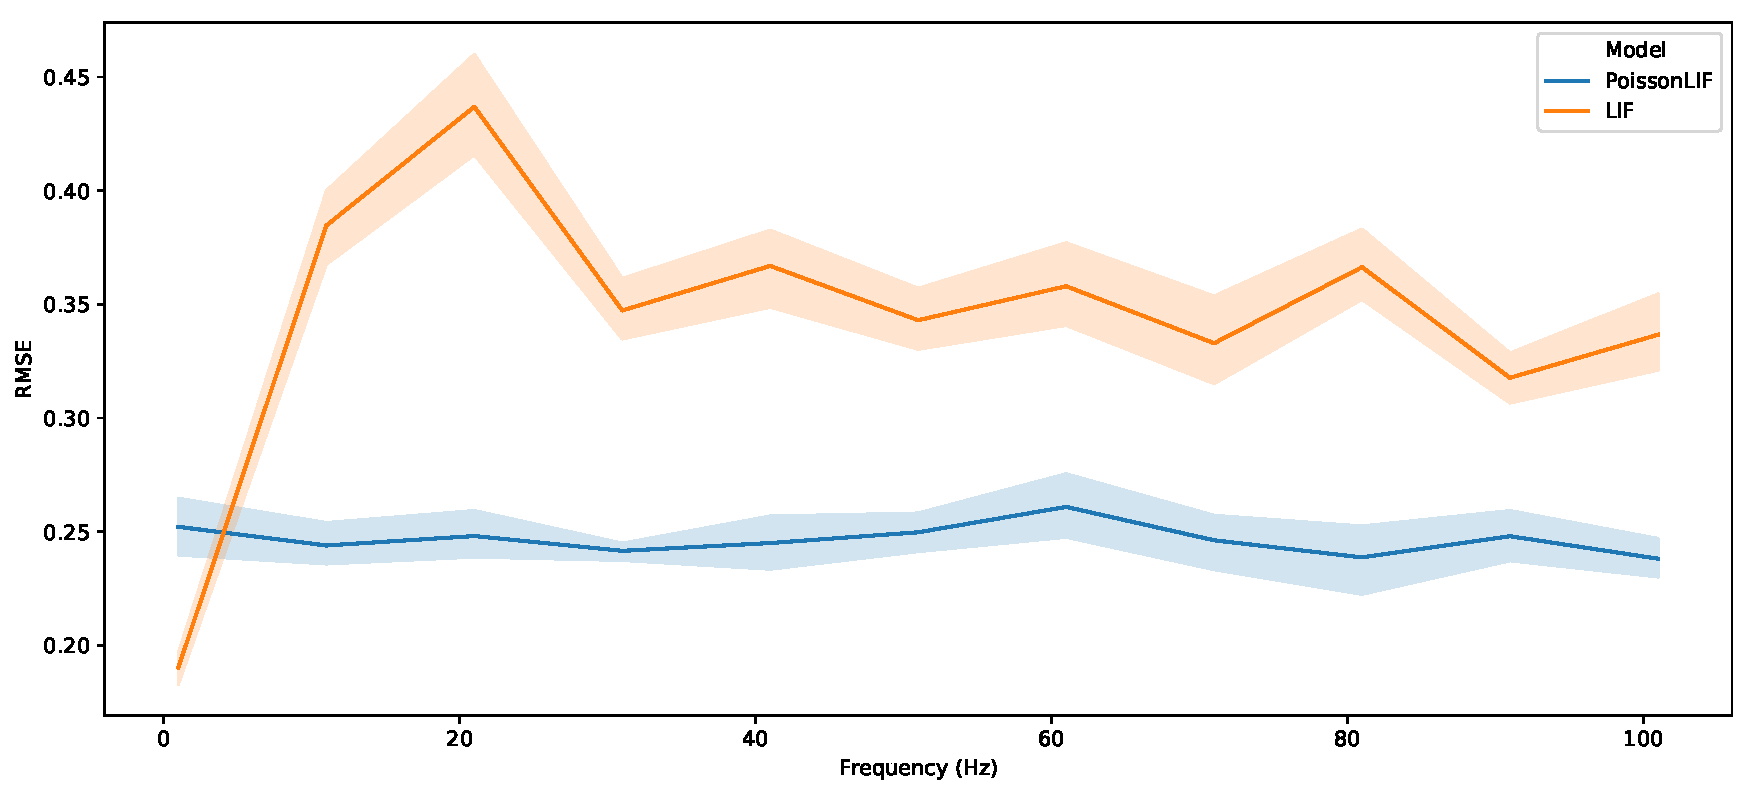
\includegraphics[width=0.9\textwidth]{poisson-frequency-scaling}
\caption[Spiking neuron performance with input frequency.]{\label{fig:poisson-frequency-scaling} Scaling of LIF performance with frequency, for each type: Poisson-spiking, non-leaky (i.e.,~integrate-and-fire), adaptive, and regular-spiking.
The input is a sinusoid with frequency $f$\,Hz.
% Both the ideal sinusoid and the decoded spike trains are filtered by $\tau = 0.01 f^{-1}$\,s to compute the RMSE.
%The number of neurons is set to $50 f$ in order to scale the total number of spikes with the input frequency, and the maximum firing rate of each neuron is uniformly distributed over $20-40$\,Hz.
%We give the LIF neurons an advantage by washing out the initial transient induced by an initial voltage of $v(0) = 0$.
Due to the memoryless property of the Poisson process, and the uniformity of ReLU, both outperform LIF with constant precision as $f \rightarrow \infty$ (Theorem~\ref{thm:correctness}), assuming $n$ and $\tau$ are scaled appropriately with frequency (see text for details).
}

\vspace{1em}

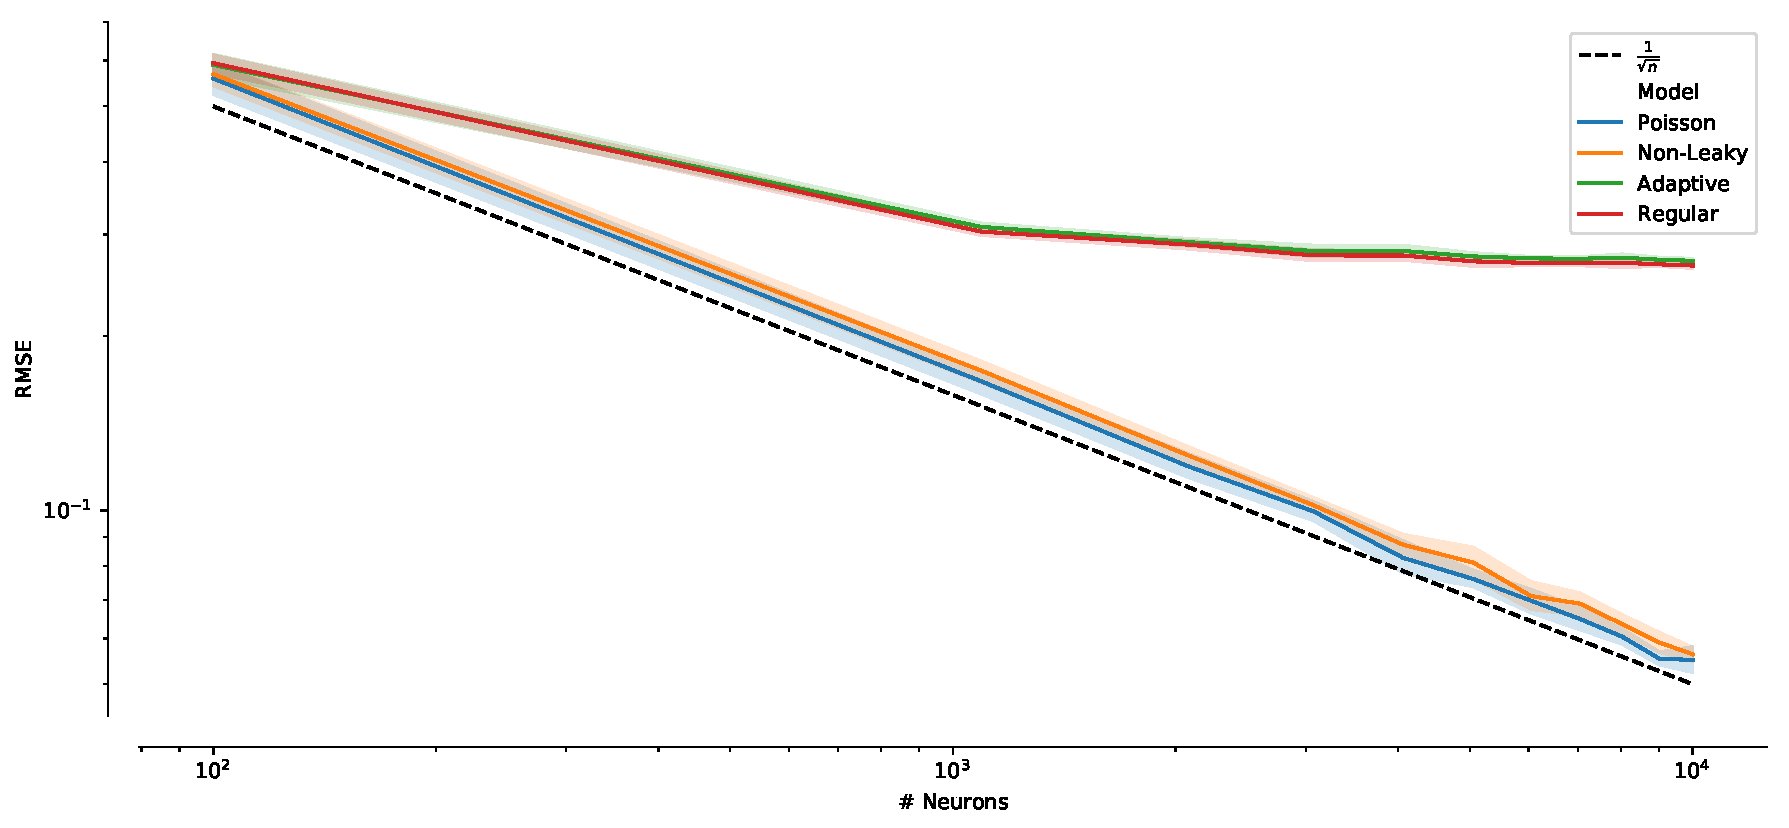
\includegraphics[width=0.9\textwidth]{poisson-neuron-scaling}
\caption[Spiking neuron performance with neuron count.]{\label{fig:poisson-neuron-scaling} Scaling of LIF performance with neuron count, for each type: Poisson-spiking, non-leaky (i.e.,~integrate-and-fire), adaptive, and regular-spiking.
%The input signal is a sinusoid with frequency $10$\,Hz, and the maximum firing rates are uniformly distributed over $20-40$\,Hz.
Regular-spiking LIF plateaus in performance for large numbers of neurons, due to the state discrepancy (definition~\ref{def:state-discrepancy}).
The precision of integrate-and-fire and Poisson-spiking both scale as ${\sqrt{n}}$ as $n \rightarrow \infty$ (Theorem~\ref{thm:correctness}), since each neuron is always ready to spike with the ideal probability. 
}
\end{figure}

We validate these claims in Figures~\ref{fig:poisson-frequency-scaling} and~\ref{fig:poisson-neuron-scaling} by using each type of LIF model---Poisson-spiking, non-leaky, adaptive, and regular-spiking---evaluating the root-mean-squared error (RMSE) against the filtered ideal.
In all cases the maximum firing rates of the neurons are limited to $20$--$40$\,Hz, and the states of the neurons are initialized to be mixed (i.e.,~uniform ISIPs).
In both figures we display 95\% confidence intervals bootstrapped from $10$ trials in each condition.

In Figure~\ref{fig:poisson-frequency-scaling}, we demonstrate that precision remains constant for both Poisson-spiking and non-leaky neurons, even at frequencies greater than six times that of the maximum firing rates of any given neuron.
For this, we set $n = 50 f$, $\tau = 10 f^{-1}$\,ms, and $\dt{} = 1 f^{-1}$\,ms, as we scale the frequency of the sinusoid, $f$\,Hz.
This choice of scaling is informed by equation~\ref{eq:psc-code-power}, which tells us that we should balance $\tau = f^{-1}$ to keep $\bigoh{2 \pi \tau f }$ fixed, while increasing $n$ in proportion to $f$ to scale the total number of spikes with frequency.
Due to the variability in a Poisson process, it is sub-optimal for constant inputs.
However, performance remains constant at higher frequencies.

In Figure~\ref{fig:poisson-neuron-scaling}, we demonstrate that the precision continues to scale as $\bigoh{\tau \sqrt{n}}$ for both Poisson-spiking and non-leaky neurons, but not for the other two.
For this, we fix $f = 10$\,Hz, $\tau = 1$\,ms, and $\dt{} = 0.1$\,ms, as we scale the neuron count.
This demonstrates that Posson spiking models (and ReLU) solve the state discrepancy problem, and thus continue to scale in accuracy with neuron count at increasingly-greater signal frequencies relative to the individual firing rates.
The properties of the Poisson neuron model make it particularly appealing for neuromorphic architectures such as SpiNNaker~2.
Specifically, SpiNNaker~2 has specialized hardware for computing exponentials~\citep{partzsch2017fixed} and uniform samples~\citep{liu2018memory}, and the architecture benefits enormously from the reduction of memory requirements and spike-traffic~\citep{stromatias2013power, mundy2015}.
Since the Poisson spike generator can be applied to any desired static response curve, this method can be applied to whatever is cheap to compute while still providing a suitable nonlinear basis for the desired transformation.

